\documentclass[12pt]{article}
\usepackage[T1]{fontenc}
\usepackage[utf8]{inputenc}
\usepackage[margin=1in]{geometry}
\usepackage[spanish]{babel}\decimalpoint
\usepackage{setspace}\onehalfspacing
\usepackage{parskip} %Espacio entre parrafos.
\usepackage{graphicx} %Para usar \includegraphics[]{}
\usepackage{amssymb} %Para usar el si­mbolo del conj. de los Reales.%
\usepackage{amsmath} % Para usar columnas vectoriales.
\usepackage{booktabs} % Para agregar \toprule y \bottomrule a tablas
\usepackage{multirow}
\usepackage{hyperref} %Siempre debe ser el ultimo paquete.


\setlength{\parindent}{0pt} %Texto justificado.
\setcounter{tocdepth}{2} %Que no incluya subsubsections en el índice.
%\setlength{\tabcolsep}{3pt}


%===================================================================%

\title{Apuntes `Calculus 1A: Differentiation'}
\author{}
\date{}

\begin{document}

\maketitle
\tableofcontents

\newpage

\section{Aplicaciones de las Derivadas.}

\subsection{Gráficos y los Puntos Críticos.}

En esta ocasión veremos cómo las derivadas nos pueden servir para visualizar cómo se comporta la gráfica de una función.

Ya sabemos que el valor y el signo (cuando es distinto de cero) de la \textbf{primera y/o segunda derivada} nos da indicios sobre cómo se está comportando una función en un punto. Ahora veremos que esta información podemos utilizarla para \textbf{dibujar bosquejos de su gráfica}.

Si bien los bosquejos no serán perfectos, va a ser suficiente como para tener una idea, por ejemplo, sobre cómo son sus curvas (concavidad o punto de esquina) a partir de \textbf{solo unos pocos puntos}.

Así, como con la ayuda del álgebra podemos saber dónde la función intersecta a los ejes X e Y o sus valores máximos y mínimos, con el cálculo tendremos conocimiento de su forma en aquellos puntos u otros.

En el siguiente cuadro tenemos un resumen de lo que nos describen la primera y segunda derivada de una función $f(x)$ en un punto $x = a$.

\begin{table}[hbt!]
\centering
{\renewcommand{\arraystretch}{1.3}
\begin{tabular}{l | l}
 & Descripción de $f(x)$ \\
\hline
$f'(a) > 0$ & $f(x)$ está \textbf{creciendo} en $x = a$ \\
$f'(a) < 0$ & $f(x)$ está \textbf{decreciendo} en $x = a$ \\
\hline
$f''(a) > 0$ & $f(x)$ es \textbf{cóncava hacia arriba} en $x = a$ \\
$f''(a) < 0$ & $f(x)$ es \textbf{cóncava hacia abajo} en $x = a$ \\
\end{tabular}
}
\end{table}


\subsubsection{Extremos Locales y Puntos Críticos.}

A lo largo de una función, podemos encontrarnos con puntos que son \textbf{mínimos y/o máximos locales}, similar a como vemos en la siguiente imagen.

\begin{figure}[hbt!]
\centering
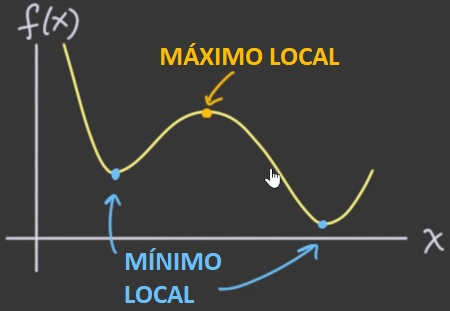
\includegraphics[scale=0.5]{img/min-max-local.jpg}
\end{figure}

La palabra \textbf{``local''} se refiere a que son valores mínimos o máximos dentro de un \textbf{intervalo de valores cercanos a dichos puntos} y no en todos los valores del dominio de la función.

Por ejemplo, en la imagen que vimos se aprecia un máximo local, pero es posible que haya otro y cuyo valor sea mayor o menor a éste. Ambos serán un máximo local, pero dentro de un rango de valores cercanos a ellos.

Formalmente, se señala que:

\begin{itemize}
\item $f(x)$ tiene un \textbf{mínimo local} en $x = a$ si $f(a) \leq f(x)$ $\forall x$ cercano a $a$.

\item $f(x)$ tiene un \textbf{máximo local} en $x = a$ si $f(a) \geq f(x)$ $\forall x$ cercano a $a$.
\end{itemize}

En conjunto, tanto un mínimo como un máximo local se denominan \textbf{extremos locales} (o \textit{local extrema}, en inglés).



\subsubsection{Prueba de la Primera Derivada.}

Como vimos, en una función es posible encontrar más de un extremo local. Estos puntos los podemos conocer a partir de su \textbf{primera derivada}.

Sabemos que cuando la \textbf{derivada} de una función $f(x)$ \textbf{es igual a cero} en $x = a$, es porque en ese lugar alcanza un valor máximo o mínimo. Es decir, estamos en presencia de un \textbf{extremo local}. No obstante, \textbf{también podemos estarlo cuando ésta no es derivable}. como cuando corresponde a un punto de esquina\footnote{Ojo que, en ambos casos, la función es continua.} (\textit{corner point}).

\begin{figure}[hbt!]
\centering
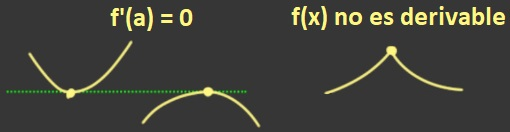
\includegraphics[scale=0.7]{img/critical-points.jpg}
\end{figure}

Ambos casos se conocen como \textbf{Puntos Críticos} de la función y su definición es la siguiente:

\begin{quote}
Si $f'(a) = 0$ o si $f$ no es derivable, entonces $a$ es un \textbf{Punto Crítico} de $f$.
\end{quote}

Esto implica que:

\begin{quote}
Todo extremo local es un punto crítico, pero no todo punto crítico es un extremo local.
\end{quote}

\newpage

Por ejemplo, en la siguiente imagen podemos ver que la función no tiene un extremo local, pero es posible apreciar que la pendiente de la línea tangente (línea verde punteada) en un punto, es igual a cero. Por lo tanto, sí corresponde a un punto crítico, pero no a un máximo o mínimo local.

\begin{figure}[hbt!]
\centering
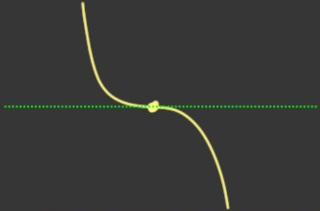
\includegraphics[scale=0.6]{img/critical-points-2.jpg}
\end{figure}

Para conocer los puntos críticos de una función, podemos aplicar lo que se denomina como la \textbf{Prueba de la Primera Derivada}.

Suponga que una función $f(x)$ tiene un punto crítico en $x = a$ y que es continua en ese lugar. La prueba de la primera derivada indica:

\begin{itemize}
\item Si $f'(a) < 0$ a la izquierda de $x = a$ y $f'(a) > 0$ a la derecha $x = a$, entonces el punto crítico es un mínimo local.

\item Si $f'(a) > 0$ a la izquierda $x = a$ y $f'(a) < 0$ a la derecha $x = a$, entonces el punto crítico es un máximo local.

\item Si $f'(a)$ tiene el mismo signo a la izquierda y a la derecha $x = a$, entonces el punto crítico no es un extremo local.
\end{itemize}

En el siguiente cuadro resumimos esta prueba.

\begin{table}[hbt!]
\centering

{\renewcommand{\arraystretch}{1.3}
\begin{tabular}{c  c  c  c}
\toprule
 & \multicolumn{3}{c}{Punto Crítico} \\
\cline{2-4}
 & Mín Local & Máx Local & Ninguno \\
\hline
Izquierda & $f'(a) < 0$ & $f'(a) > 0$ & \multirow{2}{10em}{$f'(a) < 0$ o $f'(a) > 0$ en ambos lados.} \\
\cline{2-3}
Derecha & $f'(a) > 0$ & $f'(a) < 0$ \\
\bottomrule
\end{tabular}
}

\end{table}

Entonces, para realizar la prueba de la primera derivada en una función, debemos:

\begin{enumerate}
\item Calcular su derivada.
\item Buscar todos los puntos críticos.
\item Ver qué signo toma la derivada a la izquierda y derecha de cada punto crítico.
\end{enumerate}

\textbf{Ejemplo.} \quad Busque los puntos críticos de la función $g(x) = 0.2x^{5} + 2x^{4} + 4x^{3} - 17$, determine si corresponden a extremos locales y a cuáles.

\textbf{Solución.} \quad Comencemos calculando la derivada de $g(x)$.
\[
	g'(x) = x^{4} + 6x^{3} + 12x^{2}
\]
Luego, tenemos que buscar todos los puntos críticos de $g(x)$. Para ello, factoricemos la derivada que acabamos de obtener.
\[
g'(x) = x^{2}(x^{2} + 6x + 12) = x^{2}(x + 6)(x + 2)
\]
Como la función $g(x)$ es derivable para todo $x$, sus puntos críticos serán todos aquellos donde $g'(x) = 0$.
\begin{align*}
0 &= x^{2} & 0 &= x + 6 & 0 &= x + 2 \\
0 &= x & -6 &= x & -2 &= x
\end{align*}
Veamos ahora qué signo toma $g'(x)$ en cada uno de estos puntos. Como estamos trabajando con desigualdades no lineales\footnote{En este caso, una desigualdad cuadrática.}, podemos buscar sus soluciones a partir de una \textbf{tabla de signos}.

Antes, estableceremos que $g'(x) > 0$, aunque el signo queda a discreción de cada uno, ya que veremos tanto los valores positivos como negativos de esta derivada\footnote{Esto implica que siempre trabajaremos con desigualdades estrictas, así que sus soluciones serán intervalos abiertos.}. Por lo tanto, sus soluciones son:
\[
(-\infty, \ -6) \ (-6, \ -2) \ (-2, \ 0) \ (0, \ \infty)
\]
Así, la tabla de signos será la siguiente:

\begin{table}[hbt!]
\centering

{\renewcommand{\arraystretch}{1.3}
\begin{tabular}{c c c c c}
\hline
 & $(-\infty, \ -6)$ & $(-6, \ -2)$ & $(-2, \ 0)$ & $(0, \ \infty)$ \\
\hline
$x^{2}$ & $+$ & $+$ & $+$ & $+$ \\
$x + 6$ & $-$ & $+$ & $+$ & $+$ \\
$x + 2$ & $-$ & $-$ & $+$ & $+$ \\
\hline
$x^{2}(x + 6)(x + 2)$ & $+$ & $-$ & $+$ & $+$ \\
\hline
\end{tabular}
}
\end{table}

\newpage

A partir de la tabla de signos podemos señalar:

\begin{enumerate}
\item $x = -6$ es un \textbf{máximo local}, ya que $g'(-6) > 0$ a la izquierda y $g'(-6) < 0$ a la derecha del punto crítico.

\item $x = -2$ es un \textbf{mínimo local}, ya que $g'(-2) < 0$ a la izquierda y $g'(-2) > 0$ a la derecha del punto crítico.

\item $x = 0$ \textbf{no es un extremo local}, ya que $g'(0) > 0$ a la izquierda y a la derecha del punto crítico.
\end{enumerate}


\subsubsection{Prueba de la Segunda Derivada.}

Busquemos los puntos críticos y los extremos locales de la función $f(x) = x^{2} + 3\cos(x)$.

Al calcular su derivada, obtendremos que $f'(x) = 2x - 3\sin(x)$. Esto significa que uno de sus puntos críticos será $x = 0$, puesto que $f'(0) = 2(0) - 3\sin(0) = 0$. Sin embargo, conocer si es un extremo local y de qué tipo, se vuelve más caótico.

Para evaluar si $x = 0$ es un extremo local de $f(x)$, debemos buscar todos los puntos críticos de esta función. Si bien aquello es posible, algebraicamente es bastante complicado.

Cuando se hace difícil conocer el extremo local del punto crítico de una función a partir de su primera derivada, podemos calcular la \textbf{segunda derivada} en el \textbf{punto donde la primera es igual a cero} (i.e, en el punto crítico) para \textbf{ver qué signo toma} y determinar si dicho punto es un mínimo o un máximo local. A este proceso se lo conoce como la \textbf{Prueba de la Segunda Derivada}.

%Para salir de este tipo de problemas, podemos calcular la \textbf{segunda derivada} en el punto donde la primera es igual a cero (i.e, en el punto crítico) y ver qué signo toma para determinar si dicho punto es un mínimo o un máximo local. A este proceso se lo conoce como la \textbf{Prueba de la Segunda Derivada}.

\textbf{Definición.} \quad Suponga que $f(x)$ es continua en un punto crítico $x = a$ y que $f'(a) = 0$.

\begin{itemize}
\item Si $f''(a) < 0 \rightarrow$ $x = a$ es un \textbf{máximo local} (i.e, $f(a)$ es concava hacia abajo).

\item Si $f''(a) > 0 \rightarrow$ $x = a$ es un \textbf{mínimo local} (i.e, $f(a)$ es concava hacia arriba).

\item Si $f''(a) = 0$ o $\nexists f''(a) \rightarrow$ \textbf{Prueba inconclusa}\footnote{Cuando $f''(a) = 0$ y puede seguir siendo derivada, es posible ayudarnos en la \textbf{tercera derivada}. El signo que tome nos dará información sobre la segunda y primera derivada, permitiéndonos deducir qué extremo local es el punto crítico.}: $x = a$ puede ser un mínimo o un máximo o no ser un extremo local.
\end{itemize}

\newpage

Recordemos que, geométricamente, el signo de la segunda derivada nos describe la \textbf{forma de la curva} de la función en un punto. Es decir, su \textbf{concavidad} (ver tabla en la pág. 2). Y como estamos calculándola cuando $f'(a) = 0$, entonces de inmediato sabremos si el punto crítico $x = a$ es o no un extremo local y de qué tipo, en caso de ser distinto de cero.

%\newpage

Volvamos a la función $f(x) = x^{2} + 3\cos(x)$. Ya vimos que buscar todos sus puntos críticos es bastante complicado con la primera derivada, pero al menos sabemos que $x = 0$ es uno de ellos. Por lo tanto, apliquemos la prueba de la segunda derivada en dicho punto para evaluar si es un extremo local y de qué tipo.

Al calcular la segunda derivada de $f(x)$, obtendremos que $f''(x) = 2 - 3\cos(x)$. Luego, veamos qué valor toma en $x = 0$.
\[
	f''(0) = 2 - 3\cos(0) = -1
\]
En otras palabras, la segunda derivada de $f(x)$ en $x = 0$ es \textbf{negativa}, lo que implica que en ese punto crítico es \textbf{cóncava hacia abajo} y, por consiguiente, dicho punto es un \textbf{máximo local}.

\textbf{Ejercicio.} \quad Sea $x = 0$ un punto crítico de las funciones $g(x) = x^{3}$ y $h(x) = x^{4}$, calcule la segunda derivada de ambas funciones en dicho punto y determine si es un extremo local y cuál, en los dos casos.

\textbf{Solución.} \quad Primero nos señalan que $x = 0$ es un punto crítico en $g(x)$ y en $h(x)$. Recordemos que esto se cumple si la primera derivada de ambas es igual a cero o si no es derivable en ese punto. Tanto $x^{3}$ como $x^{4}$ son derivables en el conjunto de los $\mathbb{R}$, de manera que podemos descartar la segunda opción.

Comprobemos que las derivadas de $g(x)$ y $h(x)$ sean iguales a cero en $x = 0$.
\begin{align*}
g'(0) &= 3(0)^{2} & h'(0) &= 4(0)^{3} \\
g'(0) &= 0 & h'(0) &= 0
\end{align*}
Por lo tanto, se cumple que $x = 0$ sea un punto crítico en $g(x)$ y en $h(x)$.

Ahora apliquemos la prueba de la segunda derivada para evaluar este punto crítico.

Las segundas derivadas de $g(x)$ y en $h(x)$ son, respectivamente, $g''(x) = 6x$ y $h''(x) = 12x$. Esto implica que $g''(0) = 0$ y $h''(0) = 0$. Por lo tanto, en ambos casos la prueba de la segunda derivada es \textbf{inconclusa}.

Algo que podemos hacer en este caso para ver si $x = 0$ es o no un extremo local, es tomarnos de la \textbf{definición sobre mínimo y máximo local} que vimos anteriormente\footnote{En este caso no podemos usar la tercera derivada, porque ambas resultan en una función constante.} (pág. 3).

Para ello, diremos que los valores de $x$ cercanos a cero serán todos aquellos donde $x < 0$ o $x > 0$. La idea es ver si, en dichos valores, los \textit{outputs} de las funciones son mayores o menores que $g(0) = 0$ y $h(0) = 0$.

%\newpage

Veamos los resultados en la siguiente tabla:

\begin{table}[hbt!]
\centering
{\renewcommand{\arraystretch}{1.3}
\begin{tabular}{c c c}
\hline
 & $x < 0$ & $x > 0$ \\
\hline
$g(x) = x^{3}$ & $g(x) < g(0)$ & $g(x) > g(0)$ \\
$h(x) = x^{4}$ & $h(x) > h(0)$ & $h(x) > h(0)$ \\
\hline
\end{tabular}
}
\end{table}

En el caso de $g(x)$, podemos observar que en una parte de los valores cercanos a $x = 0$, sus \textit{outputs} son menores a $g(0)$ y en la otra, mayores a dicho valor. En la definición de un extremo local se señala que aquello \textbf{se aplica a todo valor cercano de $x$} (pág. 3) y esto no ocurre acá. Por lo tanto, \textbf{$x = 0$ no es un máximo ni un mínimo local}.

En cuanto a $h(x)$, podemos verificar que en todos los valores cercanos a $x$, $h(x) > h(0)$. Por lo tanto, en esta función $x = 0$ es un \textbf{mínimo local}.


\subsubsection{Puntos de Inflexión.}

La segunda derivada también puede darnos información sobre los \textbf{lugares en donde cambia la concavidad de la función}. Aquellos en donde sí ocurre, los llamamos como \textbf{Puntos de Inflexión}.

En particular, un punto es de inflexión \textbf{si el signo de la segunda derivada cambia de un lado de éste al otro}.

Usemos, a modo de ejemplo, la función $f(x) = 2x^{6}/5 - x^{4}/4 + 7x - 2/3$.

Queremos saber en qué puntos la segunda derivada cambia de signo. Por lo tanto, lo primero que tenemos que hacer es calcularla y ver en qué valores se iguala a cero.

La primera y segunda derivada de $f(x)$, son las siguientes:
\begin{align*}
	f'(x) &= \frac{12}{5}x^{5} - x^{3} + 7 &
	f''(x) &= 12x^{4} - 3x^{2}
\end{align*}

\newpage

Factoricemos la segunda derivada de manera que sea más sencilla para trabajarla.
\[
f''(x) = 3x^{2}(4x^{2} - 1) = 3x^{2}(2x + 1)(2x - 1)
\]
Veamos ahora en qué valores cada factor de $f''(x)$ es igual a cero.
\begin{align*}
3x^{2} &= 0 & 2x + 1 &= 0 & 2x - 1 &= 0 \\
x &= 0 & x &= -\frac{1}{2} & x &= \frac{1}{2}
\end{align*}
Entonces, la idea es evaluar qué signos toma la segunda derivada tanto al lado izquierdo como derecho de estos valores de $x$. Para ello, construyamos una tabla de signos.

\begin{table}[hbt!]
\centering

{\renewcommand{\arraystretch}{1.3}
\begin{tabular}{c c c c c}
 & $(-\infty, \ -1/2)$ & $(-1/2, \ 0)$ & $(0, \ 1/2)$ & $(1/2, \ \infty)$ \\
\hline
$3x^{2}$ & $+$ & $+$ & $+$ & $+$ \\
$2x + 1$ & $-$ & $+$ & $+$ & $+$ \\
$2x - 1$ & $-$ & $-$ & $-$ & $+$ \\
\hline
$3x^{2}(2x + 1)(2x - 1)$ & $+$ & $-$ & $-$ & $+$ \\
\end{tabular}
}

\end{table}

Como se puede apreciar en la tabla de signos, la segunda derivada cambia de signo en los puntos $x = -1/2$ y $x = 1/2$, lo que quiere decir que \textbf{ambos son puntos de inflexión}, algo que no ocurre con $x = 0$, puesto que tanto a su izquierda como su derecha $f''(x) < 0$.


\subsubsection{Dibujando el bosquejo de una función.}

A partir de lo que hemos aprendido, resolvamos el siguiente ejercicio.

\textbf{Ejercicio.} \quad Sea $f(x) = x^{5}/20 + x^{4}/4$, encuentre:

\begin{itemize}
\item[a)] Las raices de la función.
\item[b)] Sus puntos críticos, evaluando si son extremos locales y cuáles.
\item[c)] Los puntos de inflexión de $f(x)$
\end{itemize}

Finalmente, a partir de esta información dibuje un bosquejo del gráfico de $f(x)$.

\textbf{Solución.} \quad Comencemos buscando las raíces de $f(x)$, igualándola a cero.
\[
0 = \frac{x^{5}}{20} + \frac{x^{4}}{4} =
	\frac{x^{4}}{4} \left(\frac{x}{5} + 1\right)
\]
Como vemos, hay dos posibles valores, los que podemos encontrar a continuación:
\begin{align*}
0 &= \frac{x^{4}}{4} & 0 &= \frac{x}{5} + 1 \\
0 &= x & -5 &= x
\end{align*}
Por consiguiente, la curva de $f(x)$ corta al eje X en $x = 0$ y $x = -5$.

Ahora busquemos los puntos críticos de $f(x)$. Para ello, calculemos su derivada.
\[
f'(x) = \frac{x^{4}}{4} + x^{3} = \frac{x^{3}}{4} (x + 4)
\]
Igualemos a cero los factores de esta derivada, para encontrar sus puntos críticos.
\begin{align*}
0 &= \frac{x^{3}}{4} & 0 &= x + 4 \\
0 &= x & -4 &= x
\end{align*}
Veamos si ambos puntos críticos son extremos locales y de qué tipo a partir de una tabla de signos.

\begin{table}[hbt!]
\centering

{\renewcommand{\arraystretch}{1.3}
\begin{tabular}{c c c c}
 & $(-\infty, \ -4)$ & $(-4, \ 0$) & $(0, \ \infty)$ \\
\hline
$x^{3}/4$ & $-$ & $-$ & $+$ \\
$x + 4$ & $-$ & $+$ & $+$ \\
\hline
$x^{3}/4 (x + 4)$ & $+$ & $-$ & $+$ \\
\end{tabular}
}

\end{table}

A partir de la tabla de arriba podemos concluir que ambos puntos son extremos locales, donde $x = -4$ es un máximo local y $x = 0$ un mínimo local.

Ahora veamos si $f(x)$ tiene puntos de inflexión.

La segunda derivada de $f(x)$ es la siguiente:
\[
f''(x) = x^{3} + 3x^{2} = x^{2}(x + 3)
\]
Como volveremos a usar la tabla de signos, igualemos a cero los factores de $f''(x)$.
\begin{align*}
0 &= x^{2} & 0 &= x + 3 \\
0 &= x & -3 &= x
\end{align*}
Luego, construyamos la tabla de signos para evaluar si $f(x)$ tiene o no puntos de inflexión.

\begin{table}[hbt!]
\centering

{\renewcommand{\arraystretch}{1.3}
\begin{tabular}{c c c c}
 & $(-\infty, \ -3)$ & $(-3, \ 0$) & $(0, \ \infty)$ \\
\hline
$x^{2}$ & $+$ & $+$ & $+$ \\
$x + 3$ & $-$ & $+$ & $+$ \\
\hline
$x^{2}(x + 3)$ & $-$ & $+$ & $+$ \\
\end{tabular}
}

\end{table}

%\newpage

De este modo, podemos decir que solo $x = -3$ es un punto de inflexión de $f(x)$.

Ahora solo nos queda dibujar un bosquejo de la gráfica. Resumamos la información que manejamos hasta ahora.

\begin{itemize}
\item Raíces de $f(x) \rightarrow$ $x = -5$ y $x = 0$.
\item Puntos críticos de $f(x) \rightarrow$ $x = -4$ (máx. local) y $x = 0$ (mín. local).
\item Punto de inflexión de $f(x) \rightarrow$  $x = -3$, donde $f''(x) > 0$ en $x \geq -3$.
\end{itemize}

A continuación tenemos el bosquejo de $f(x)$ dibujado con la información recabada.% que está resumida arriba.

\begin{figure}[hbt!]
\centering
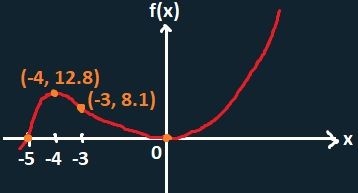
\includegraphics[scale=0.7]{img/final-draft-plot-2.jpg}
\end{figure}

Si bien no es una representación perfecta, es muy similar a la gráfica original de $f(x)$.

\begin{figure}[hbt!]
\centering
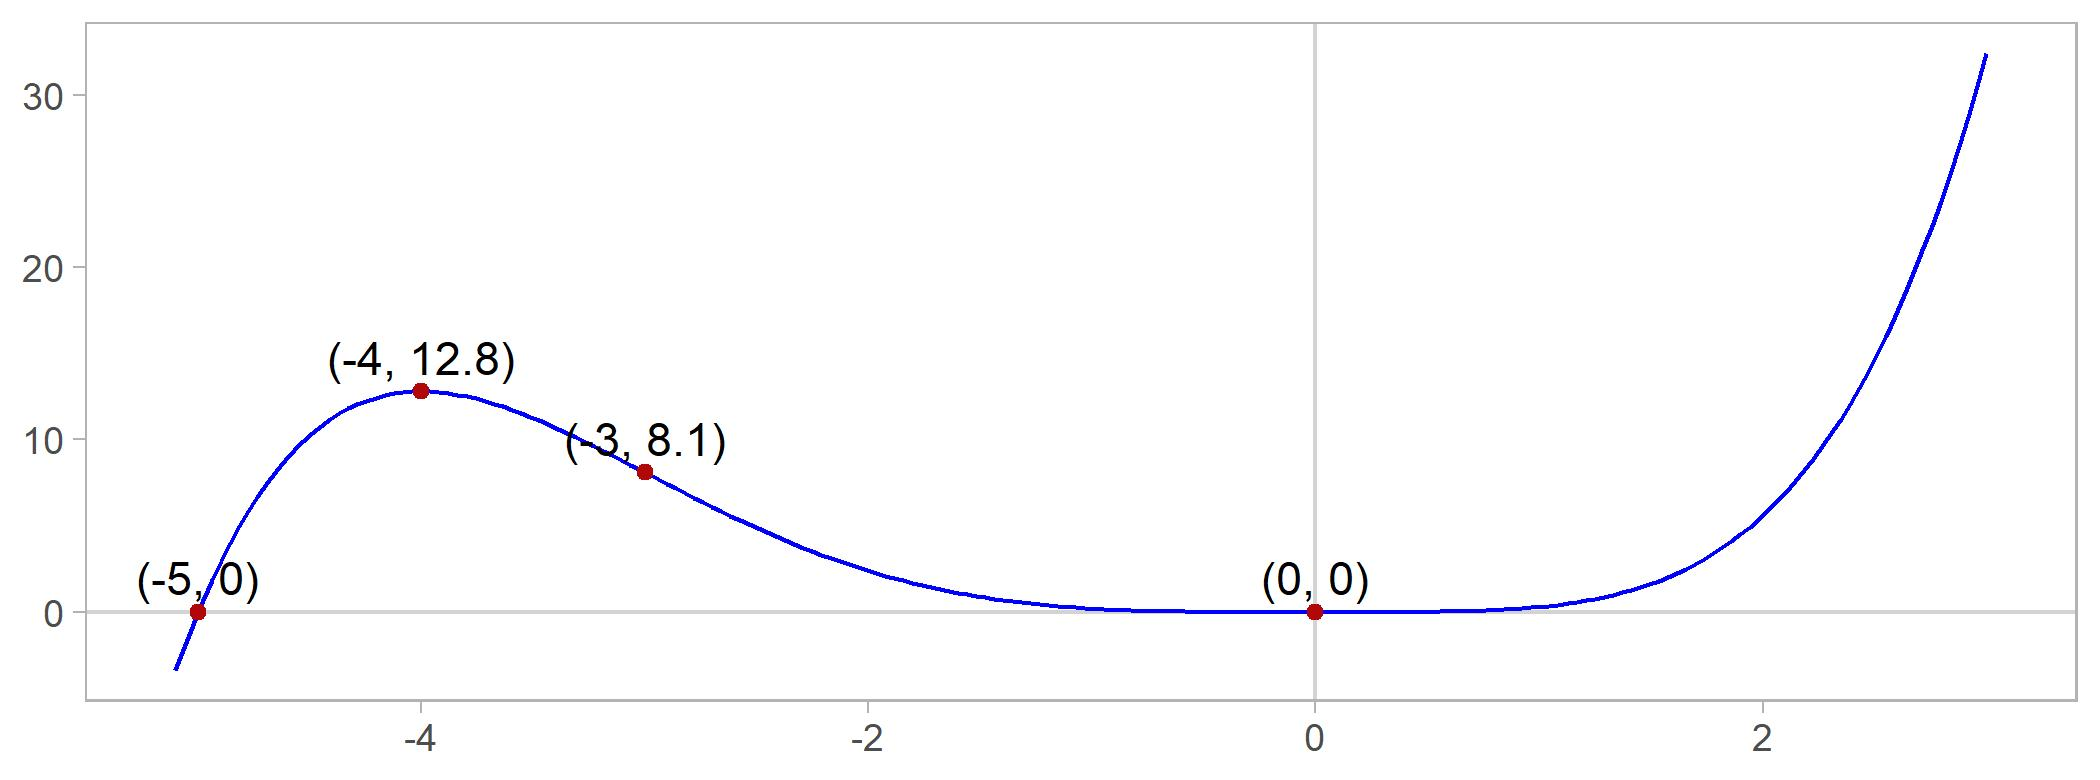
\includegraphics[scale=0.7]{img/final_draft_original.jpg}
\end{figure}

\newpage


\subsection{La Gran Imagen: Límites y Asíntotas.}

En la sección anterior, vimos cómo la primera y segunda derivada de una función pueden ayudarnos para conocer su comportamiento a lo largo de su dominio, dibujando un bosquejo de su curva. Sin embargo, en aquella ocasión no consideramos los casos cuando ésta tiene \textbf{discontinuidades} y si es \textbf{asíntota vertical} o no en dichos lugares. Del mismo modo, tampoco sabemos cuál es su conducta en los extremos de su dominio. En otras palabras, también es posible encontrarnos con \textbf{asíntotas horizontales}.

Para estudiar las asíntotas de una función, calcularemos sus límites. En el caso de las discontinuidades y las asíntotas verticales, retomaremos lo que vimos en la primera semana sobre \textbf{límites infinitos} (\textit{infinite limits}). A ésto, incluiremos como nuevo material los \textbf{límites en el infinito} (\textit{limits at infinity}), que es cuando queremos saber dichos valores a medida que $x \to \pm \infty$. También veremos qué hacer cuando los límites son de la forma $0/0$ o $\infty/\infty$, donde para resolverlas utilizaremos la \textbf{regla de L'Hôspital}.

Con todo esto, tendremos las herramientas suficientes para dibujar bosquejos aún más precisos sobre nuestras funciones de interés.


\subsubsection{Asíntotas Verticales y Horizontales.}

Antes de volver a meternos en los bosquejos de gráficos, centrémonos en cómo encontrar asíntotas. Es decir, en los límites infinitos y en el infinito\footnote{Esta subsección no está en el curso y la agregué para profundizar un poco sobre las asíntotas horizontales. Me baso un poco en lo visto en la Semana 1 del curso y en el libro \textit{Cálculo de una variable. Trascendentes tempranas} de James Steward (6ta Edición, 2008). Por otra parte, decidí trabajar los límites desde su entendimiento ``informal'', para avanzar más rápido. Otro libro que recomiendo para profundizar, es \textit{Cálculo de una variable} de George Thomas.}.

En la primera semana del curso, vimos que cuando el límite de una función en un punto era igual a $\pm \infty$, significaba que en ese lugar no existe un límite porque \textbf{la función era asíntota vertical} hacia arriba o abajo, según el signo (ver \href{../week-1/week_1.pdf}{págs. 40-45}). En particular, nos concentramos en los límites de funciones racionales cuyo su resultado en un punto era de la forma $a/0$, $\{\forall a \in \mathbb{Z} \ | \ a \neq 0\}$.

Por ejemplo:
\[
	\lim_{x \to 3^{+}} \frac{2x}{x - 3} =
	\frac{6}{0^{+}} = 
	\infty
\]
puesto que, a medida que $x \to 3^{+}$, $2x \to 6$ y $x - 3 \to 0$. Por otra parte, es ``positivo''\footnote{El infinito no es un número, pero por fines ilustrativos se dice su signo.} porque el numerador y el denominador son del mismo signo.

\newpage

Pero las asíntotas verticales no son exclusivas de las funciones racionales. Otro ejemplo puede ser $\lim_{x \to 0^{+}} \ln(x)$. Veamos en la siguiente tabla cómo se comporta esta función a medida que nos acercamos a $0^{+}$.

\begin{table}[hbt!]
\centering

{\renewcommand{\arraystretch}{1.3}
\begin{tabular}{c | c c c c c}
$x$ & 0.05 & 0.01 & 0.005 & 0.001\\
\hline
$\approx \ln(x)$ & $-2.996$ & $-4.6052$ & $-5.2983$ & $-6.908$
\end{tabular}
}

\end{table}

Como se puede apreciar, el $\ln(x)$ simplemente va creciendo (lentamente) hacia valores negativos a medida que $x \to 0^{+}$, pero nunca hacia un número en particular. Por lo tanto, el $\lim_{x \to 0^{+}} \ln(x) = -\infty$. Esto significa que dicho \textbf{límite no existe} y se debe a que la función $\ln(x)$ es \textbf{asíntota vertical} en $x = 0$.

Debido a la posible existencia de las asíntotas verticales, siempre es relevante revisar si existen \textbf{discontinuidades} en algunos puntos y ver cómo se comporta al acercarse a ellas\footnote{En la función $\ln(x)$, su discontinuidad está en $x = 0$ porque no está definida en dicho lugar y constatamos que se debe a que tiende al $-\infty$.}.

Pero así como una función puede ser asíntota vertical, también puede serlo de forma \textbf{horizontal}.

Las \textbf{asíntotas horizontales} existen cuando, al aproximar arbitrariamente el input de una función hacia un número muy grande en magnitud (la expresión que se usa en esos casos, es el $\pm \infty$), su output se acerca a un determinado valor.

Es decir, si existe el \textbf{límite al infinito} de una función $f(x)$ como se ve a continuación:
\[
	\lim_{x \to -\infty} f(x) = L
	\quad \text{o} \quad
	\lim_{x \to \infty} f(x) = L
\]
entonces la recta $y = L$ es la asíntota horizontal de $f(x)$.

Una diferencia con la asíntota vertical, es que una función puede intersectar en numerosas ocasiones a la recta de la asíntota horizontal, principalmente porque el límite que se obtiene es cuando $x$ se acerca a sus extremos $\pm \infty$. Por lo tanto, es poco relevante que intersecte en valores más alejados, pero sí lo es cuando está cerca del infinito.

%Lo que nos indica el límite al infinito es que, al acercarnos a un número muy grande, la función pasa tender a un valor.

Para calcular el límite al infinito de una función, podemos aplicar las leyes vistas en la semana 1 (ver \href{../week-1/week_1.pdf}{págs. 13-16 y págs. 31-39}) sumado a la siguiente:

Si $r$ es un número racional positivo, entonces:
\[\lim_{x \to \infty} \frac{1}{x^{r}} = 0\]

\newpage

Si $r$ es un número racional positivo tal que $x^{r}$ está definida para toda $x$, entonces:
\[\lim_{x \to -\infty} \frac{1}{x^{r}} = 0\]
Lo que nos dice esta propiedad es que, cuando el denominador toma valores muy grandes en magnitud, la función se acerca a cero.
Es muy útil tenerlo en cuenta cuando calculamos límites al infinito de funciones racionales con polinomios en sus numeradores y/o denominadores.

\textbf{Ejercicio.} \quad Evalúe el límite cerca de $x = \pm \infty$ de la función $f(x) = (x - 2)^{4}(x + 1)^{3}(x - 1)$.

\textbf{Solución.} \quad Por lo general, este tipo de límites se resuelven de forma intuitiva.

Podemos observar que en los tres factores de $f(x)$, todos tenderán al infinito y, por consiguiente, ya podemos deducir esa es la respuesta de este ejercicio, pero siempre es bueno analizar un poco más.

Por ejemplo, si apostamos por cuál factor será determinante en que $f(x) \to \infty$, la mejor opción es $(x - 2)^{4}$, puesto que siempre será 4 veces la resta de su paréntesis para cualquier valor de $x$. En cambio, los otros factores serán 3 y 1 vez. Es decir, crecerán más lento en comparación al primer factor. En ese sentido, podemos establecer que:
\[\lim_{x \to \infty} f(x) = \infty\]
Veamos ahora qué debe ocurrir con $f(x)$ cuando $x \to -\infty$, donde el caso es menos obvio. Digamos que $x = -\infty$ es un valor numérico muy grande, por lo tanto:
\[f(-\infty) = (-\infty - 2)^{4}(-\infty + 1)^{3}(-\infty - 1)\]
Esto implica que:
\begin{align*}
(-\infty - 2)^{4} &> 0 &
(-\infty + 1)^{3} &< 0 &
(-\infty - 1) &< 0
\end{align*}
Si multiplicamos los factores, deberíamos obtener que $f(-\infty) > 0$. Bajo este razonamiento podemos concluir que:
\[\lim_{x \to -\infty} f(x) = \infty\]
En otras palabras, el límite al infinito no está definido en $f(x)$ y, por consiguiente, no es asíntota horizontal.

\newpage

\textbf{Ejercicio.} \quad Evalúe el siguiente límite:
\[
	\lim_{x \to \infty} \frac{3x^{2} - x - 2}{5x^{2} + 4x + 1}
\]
\textbf{Solución.} \quad Cuando evaluamos límites al infinito de polinomios de mayor grado, siempre es bueno considerar la variable de mayor grado, puesto que es la que será determinante en el valor que tome la función a medida que $x$ se acerca al infinito.

Ahora bien, en este ejercicio estamos trabajamos con una función racional, donde el numerador y el denominador son polinomios. Evaluar de forma intuitiva su límite al infinito se hace más complejo, porque no tenemos cómo saber qué ocurre con la proporción. Simplemente intuímos que tanto el numerador como el denominador crecerán a un número muy grande, pero no sabemos en qué resultará.

En estos casos, una buena estrategia es dividir tanto el numerador como el denominador por el término de mayor orden de ambas expresiones. En este ejercicio es $x^{2}$. Por consiguiente:
\[
	\lim_{x \to \infty}
		\left(
			\left. \frac{3x^{2} - x - 2}{x^{2}} \right/
			\frac{5x^{2} + 4x + 1}{x^{2}}
		\right)
\]
Al simplificar las fracciones del numerador y denominador, obtendremos los siguiente:
\[
	\lim_{x \to \infty}
		\left(
			\left. 3 - \frac{1}{x} - \frac{2}{x^{2}} \right/
			5 + \frac{4}{x} + \frac{1}{x^{2}}
		\right)
\]
Como podemos observar, al aplicar el límite a cada expresión del numerador y del denominador, en algunas de ellas es posible aplicar la propiedad que vimos anteriormente (págs. 13-14), resultando en lo que sigue:
\[
	\lim_{x \to \infty}
		\left(
			\left. 3 - \frac{1}{x} - \frac{2}{x^{2}} \right/
			5 + \frac{4}{x} + \frac{1}{x^{2}}
		\right) =
		\frac{3 - 0 - (2 \cdot 0)}{5 + (4 \cdot 0) + 0} =
		\frac{3}{5}
\]
Entonces, cuando evaluamos el límite al infinito de una función racional con polinomios de alto orden en su numerador y denominador, siempre es bueno aplicar algo de álgebra para saber cómo se comporta y si es que tiene un límite definido o no.

\newpage

\subsubsection{Bosquejo de gráficos: Discontinuidades y Puntos finales.}

Volvamos a concentrarnos en los bosquejos de gráficos a partir de la siguiente función\footnote{Desde acá en adelante, los apuntes corresponden al curso.}:
\[
	f(x) = \frac{x + 1}{x + 2}
\]
Debido a que usamos la primera y segunda derivada para dibujar su bosquejo, a continuación las tenemos calculadas para $f(x)$.
\begin{align*}
	f'(x) &= \frac{1}{(x + 2)^{2}} &
	f''(x) &= \frac{2}{(x + 2)^{2}}
\end{align*}
Como recordaremos, para saber si una función tiene puntos críticos, vemos en qué valores su primera derivada es igual a cero. Sin embargo, sucede que $f'(x)$ nunca será igual a cero, lo que implica que $f(x)$ no tiene puntos críticos. Lo mismo ocurre con los puntos de inflexión, puesto que su segunda derivada tampoco será igual a cero en algún valor de $x$.

En otras palabras, estamos en un contexto donde no podemos graficar el bosquejo de $f(x)$ como lo hacíamos en la sección anterior. No obstante, en esa ocasión no revisamos si tenían discontinuidades y, de haberlas, si eran \textbf{asíntotas verticales} en dichos lugares. Tampoco evaluamos la existencia de \textbf{asíntotas horizontales} por medio de sus puntos finales. Esta información también es útil para conocer la gráfica de una función y la comenzaremos a integrar a partir de este ejercicio.

En primer lugar, es posible notar que $f(x)$ tiene una discontinuidad en $x = -2$, puesto que ahí el denominador se iguala cero. Por lo tanto, podemos evaluar su límite en aquel lugar para ver si es asíntota vertical en ese punto.
\begin{align*}
\lim_{x \to -2^{-}} \frac{x + 1}{x + 2} &= 
		\frac{-2 + 1}{-2 + 2}
		= \frac{-1}{0^{-}}
		= \infty
&
\lim_{x \to -2^{+}} \frac{x + 1}{x + 2} &= 
		\frac{-2 + 1}{-2 + 2}
		= \frac{-1}{0^{+}}
		= -\infty
\end{align*}
Entonces, al acercarnos a $x = -2$ desde la izquierda, $f(x)$ es asíntota vertical hacia arriba. Y cuando lo hacemos desde la derecha, es asíntota vertical hacia abajo.

En cuanto a conocer los puntos finales de $f(x)$, nos referimos a evaluar la existencia de asíntotas verticales a partir de los límites al infinito negativo y positivo.

Como $f(x)$ es una función racional, dividamos por $x$ tanto el numerador como el denominador para poder saber qué ocurre con aquella división a medida que nos acercamos al infinito.
\[
	f(x) = \frac{x + 1}{x + 2} =
	       \frac{(x + 1)/x}{(x + 2)/x} =
	       \frac{1 + (1/x)}{1 + (2/x)}
\]
Luego, evaluemos sus límites.
\begin{align*}
\lim_{x \to -\infty} \left(\frac{1 + (1/x)}{1 + (2/x)}\right) &=
	\frac{1 + 0}{1 + (2 \cdot 0)} = 1
&
\lim_{x \to \infty} \left(\frac{1 + (1/x)}{1 + (2/x)}\right) &=
	\frac{1 + 0}{1 + (2 \cdot 0)} = 1
\end{align*}
Por lo tanto, $f(x)$ se hace asíntota horizontal en $y = 1$ cuando $x \to \pm \infty$.

Una pregunta que puede surgirnos es si $f(x)$ va a intersectar a la asíntota horizontal $y = 1$. Para que eso ocurra, debería tener mínimos o máximos locales (al menos uno de ellos), pero sabemos que no existen, porque $f'(x)$ nunca va a ser igual a cero. Por lo tanto, la gráfica de $f(x)$ nunca intersectará a $y = 1$.

Antes de dibujar el bosquejo, veamos cuáles son las raíces (1) y el punto de intersección con el eje Y (2) de $f(x)$.
\begin{align*}
(1) \ 0 &= \frac{x + 1}{x + 2} & (2) \ f(0) &= \frac{0 + 1}{0 + 2} \\
	 -1 &= x & f(0) &= 0.5
\end{align*}
Por consiguiente, $f(x)$ intersecta al eje X en el punto $(-1, \ 0)$ y al eje Y en $(0, \ 0.5)$. De este modo, estamos en condiciones de dibujar el bosquejo de $f(x)$.

\begin{figure}[hbt!]
\centering
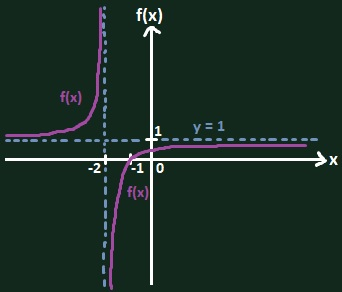
\includegraphics[scale=0.85]{img/draft-asymptote.jpg}
\end{figure}

\newpage

Para terminar, veamos la siguiente \textbf{estrategia para graficar bosquejos de funciones}:

\begin{enumerate}

\item Identificar discontinuidades (especialmente las infinitas), puntos finales (cuando $x \to \pm \infty$) y puntos fáciles (i.e, cuando $x = 0$ e $y = 0$).

\item Ver la existencia de puntos críticos y sus valores, revisando en primera instancia si $f'(x) = 0$ o si no está definida; y evaluar si $f(x) < 0$ o $f(x) > 0$ entre estos puntos. También se recomienda hacerlo para los puntos finales y las discontinuidades, como un doble chequeo.

\item Calcular $f''(x)$ para evaluar la concavidad de $f(x)$ (i.e, si $f''(x) < 0$ o $f''(x) > 0$), sobre todo como un doble chequeo para los extremos locales. También es posible usarla para revisar cambios en su concavidad, identificando sus puntos de inflexión.

\item Usar toda esta información para graficar la función.

\end{enumerate}


\subsubsection{Regla de L'Hôspital.}

Intentemos graficar un bosquejo de la siguiente función:
\[
	f(x) = \frac{x - 1}{\ln(x)}
\]
Debido al $\ln(x)$ en el denominador, $f(x)$ no está definida en $x = 0$ ($\ln(0)$ no existe) y en $x = 1$ (la fracción se divide por cero). Es decir, el dominio de $f(x)$ podemos denotarlo como:
\[
(0, \ 1) \cup (1, \ \infty) \quad \text{o} \quad 
\{x \ | \ 0 < x < 1, \ 1 < x < \infty\}
\]
Esto también nos dice que tenemos dos discontinuidades: $x = 0$ y $x = 1$. Por lo tanto, podemos evaluar si van al infinito calculando el límite cerca ambos lugares.
\begin{align*}
\lim_{x \to 0^{+}} \frac{x - 1}{\ln(x)} &=
	\frac{-1}{-\infty} = 0 \\ \\
\lim_{x \to 1} \frac{x - 1}{\ln(x)} &=
	\frac{0}{0} = \text{??}
\end{align*}
Como podemos observar, tenemos un problema con el $\lim_{x \to 1} f(x)$, porque no sabemos hacia dónde se aproxima. Cuando esto ocurre, se señala que \textbf{el límite tiene una forma indeterminada}.

En esta ocasión, nos interesan dos formas indeterminadas:
\begin{equation*}
\frac{0}{0} \quad \text{o} \quad \frac{\infty}{\infty}
\end{equation*}
Si bien no sabemos qué está ocurriendo en ambas fracciones, con la ayuda de \textbf{derivadas} veremos que podemos tener más certeza de los límites a los que se aproximan las funciones. A este procedimiento, se lo conoce como la \textbf{Regla de L'Hôspital}.

La \textbf{regla de L'Hôspital} es un método sistemático que utiliza derivadas para evaluar límites de las formas indeterminadas $0/0$ y $\infty / \infty$. Su definición es como sigue:

Sean $h(x) = f(x)/g(x)$ y $a$ un número tal que $a \in \mathbb{R}$. A medida que $x \to a$,
\begin{align*}
\text{si } f(x) \to 0 \text{ y } g(x) \to 0
\quad \text{o} \quad
\text{si } f(x) \to \infty \text{ y } g(x) \to \infty
\end{align*}
Entonces:
\[
\lim_{x \to a} \frac{f(x)}{g(x)} = \lim_{x \to a} \frac{f'(x)}{g'(x)}
\]
Si y solo si:

\begin{itemize}
\item $f(x)$ y $g(x)$ sean derivables cerca de $x = a$.

\item Y si el límite del cuociente de las derivadas existe o si se aproxima a $\pm \infty$.
\end{itemize}

Algunos aspectos interesantes de la regla de L'Hôspital, es que sea $a^{+}$ o $a^{-}$, el límite de las derivadas del numerador y del denominador se mantiene para ambas formas indeterminadas. Lo mismo ocurre si $a$ es reemplazado por $\pm \infty$ (hasta ahora solo hemos asumido que $a$ es un número finito).

Volvamos al ejemplo de $f(x) = (x - 1)/\ln(x)$. Vimos que $\lim_{x \to 1} f(x) = 0/0$, pero debido a que tiene esta forma indeterminada y que el numerador como el denominador son derivables, tenemos la opción de aplicar la regla de L'Hôspital.
\[
\lim_{x \to 1} \frac{(x - 1)'}{(\ln(x))'} =
\lim_{x \to 1} \frac{1}{1/x} =
\lim_{x \to 1} x = 1
\]
En consecuencia, como $f(x)$ no tiende al infinito cerca de $x = 0$ y $x = 1$, podemos concluir que no es asíntota vertical en ninguno de los dos lugares.

No continuaré con el bosquejo de $f(x)$, pero si las ganas persisten, dejo tres pistas: No es asíntota horizontal; tanto su primera como segunda derivada no pueden ser iguales a cero y su forma está determinada en gran medida por $\ln(x)$.

\subsubsection{Justificación de la Regla de L'Hôspital para la forma $0/0$.}

Veamos a continuación cómo podemos justificar la regla de L'Hôspital para el límite con forma indeterminada $0/0$.

Supongamos que estamos calculando:
\[
	\lim_{x \to a} \frac{f(x)}{g(x)} \quad
	\text{donde } a \in \mathbb{R}
\]
y nos encontramos en un contexto donde  $f(a) = g(a) = 0$. En otras palabras:
\[
	\lim_{x \to a} \frac{f(x)}{g(x)} = \frac{0}{0}
\]
Un camino que podemos tomar sin alterar este cuociente entre las dos funciones es, primero, multiplicar el numerador y el denominador por $1/(x-a)$.
\[
	\lim_{x \to a} \frac{f(x)/(x - a)}{g(x)/(x - a)}
\]
Y, en segundo lugar, podemos restar el numerador de $f(x)/(x - a)$ por $f(a)$. Del mismo, es posible hacerlo con $g(a)$ en $g(x)/(x - a)$, puesto que $f(a) = g(a) = 0$.
\[
	\lim_{x \to a} \frac{f(x) - f(a)/(x - a)}{g(x) - g(a)/(x - a)}
\]
Aplicando la ley del cuociente para los límites a la expresión de arriba, entonces:
\[
\left(
	\left.
	\lim_{x \to a} \frac{f(x) - f(a)}{x - a}
	\right/
	\lim_{x \to a} \frac{g(x) - g(a)}{x - a}
\right) =
\frac{f'(a)}{g'(a)}
\]
Por lo tanto, podemos señalar que:
\[
	\lim_{x \to a} \frac{f(x)}{g(x)} = 
	\lim_{x \to a} \frac{f'(x)}{g'(x)} = 
	\frac{f'(a)}{g'(a)}
	\iff
	f(a) = g(a) = 0 \text{ y }
	g'(a) \neq 0
\]
Otra forma de justificar la regla de L'Hôspital para la forma $0/0$, es calculando la aproximación lineal tanto en el numerador como el denominador de la función cerca de $x = a$.
\[
\frac{f(x)}{g(x)} \approx
	\frac{f(a) + f'(a)(x - a)}{g(a) + g'(a)(x - a)}
\]

\newpage

Como estamos trabajando bajo el supuesto de que $f(a) = g(a) = 0$, por lo tanto:
\[
	\frac{0 + f'(a)(x - a)}{0 + g'(a)(x - a)} = 
	\frac{f'(a)(x - a)}{g'(a)(x - a)} = 
	\frac{f'(a)}{g'(a)}
\]
En definitiva, lo que nos está diciendo esta regla es que \textbf{si existe el límite del cuociente entre las dos derivadas, entonces también lo hace el límite anterior}. Esto es muy relevante para el siguiente ejemplo.

Sea: 
\[
	\lim_{x \to 0} \frac{\cos(x) - 1}{x^{2}} = \frac{0}{0}
\]
Debido a que es de la forma indeterminada $0/0$ y a que el numerador y el denominador son derivables, podemos aplicar la regla de L'Hôspital. Sin embargo, como veremos a continuación, también nos lleva a la forma $0/0$.
\[
	\lim_{x \to 0} \frac{\cos(x) - 1}{x^{2}} =
	\lim_{x \to 0} \frac{-\sin(x)}{2x} =
	\frac{0}{0}
\]
La idea de la regla de L'Hôspital, es verificar la existencia de los límites de las formas $0/0$ y $\infty/\infty$. En caso de volver a toparnos con ellas, \textbf{podemos aplicar otra vez esta regla} siempre que podamos seguir derivando tanto el numerador como el denominador.

Por lo tanto:
\[
	\lim_{x \to 0} \frac{\cos(x) - 1}{x^{2}} =
	\lim_{x \to 0} \frac{-\sin(x)}{2x} =
	\lim_{x \to 0} \frac{-\cos(x)}{2} =
	-\frac{1}{2} = -0.5
\]
Este resultado nos dice que existen los dos límites anteriores y que son iguales a $-0.5$.

\subsubsection{Aplicando la regla de L'Hôspital a otras formas indeterminadas.}

\subsubsection*{a) \underline{Casos}: $0 \cdot \infty$ y $\infty - \infty$.}

Al calcular límites también es posible que nos encontremos con otras formas indeterminadas. Veamos estos dos casos:
\begin{align*}
\text{(1) Si }& \lim_{x \to a} f(x) = 0 \text{ y }
			   \lim_{x \to a} g(x) = +\infty \Longrightarrow 
			   \lim_{x \to a} f(x)g(x) = 0 \cdot +\infty \\
\text{(2) Si }& \lim_{x \to a} f(x) = \lim_{x \to a} g(x) = + \infty
			   \Longrightarrow
			   \lim_{x \to a}(f(x) - g(x)) = \infty - \infty
\end{align*}
En ambos casos no sabemos a qué valores se están acercando. Por ejemplo, en $0 \cdot +\infty$ no podemos deducir si el límite está yendo a un número muy grande o muy pequeño, porque no tenemos idea alguna sobre qué es $+\infty$. Del mismo modo ocurre con $\infty - \infty$. Tampoco podemos especular cuál es el valor que es determinante en ambos casos.

Afortunadamente, en estos casos también podemos usar la regla de L'Hôspital, pero tenemos que aplicar un poco de álgebra a las funciones de manera que se cumpla que sus límites al ser evaluados, sean de la forma $0/0$ o $\infty/\infty$.

\textbf{Ejercicio.} \quad Sea $h(x) = x\ln(x)$, evalúe su límite cerca de $x = 0^{+}$.

\textbf{Solución.} \quad Al evaluar el límite de $h(x)$ a medida que $x$ se acerca a $0^{+}$, obtenemos la siguiente forma indeterminada.
\[
\lim_{x \to 0^{+}} x \ln(x) = 0 \cdot (-\infty)
\]
Sin embargo, podemos usar un poco de álgebra para poder aplicar la regla de L'Hôspital.

Un camino a seguir es representar el $x$ del producto de $h(x)$ como $1/x$, ya que la expresión se mantiene intacta.
\[h(x) = x \cdot \ln(x) = \frac{\ln(x)}{1/x} \]
Al evaluar el límite otra vez cerca de $x = 0^{+}$, logramos la forma indeterminada de nuestro interés.
\[
	\lim_{x \to 0^{+}} \frac{\ln(x)}{1/x} = \frac{-\infty}{\infty}
\]
Por lo tanto, es posible aplicar la regla de L'Hôspital y conocer el valor al cual se acerca $h(x)$.
\[
	\lim_{x \to 0^{+}} \frac{\ln(x)}{1/x} =
	\lim_{x \to 0^{+}} \frac{1/x}{-1/x^{2}} =
	\lim_{x \to 0^{+}} -x = 0
\]
\textbf{Ejercicio.} \quad Calcule $\lim_{x \to \pi/2} \sec(x) - \tan(x)$.

\textbf{Solución.} \quad Si evaluamos el límite, veremos que:
\[
\lim_{x \to \pi/2} \sec(x) - \tan(x) = \infty - \infty
\]
Esto se debe, principalmente, a que en ambas funciones su denominador es el $\cos(x)$ y el $\cos(\pi/2) = 0$. Veamos si a partir de las fórmulas de la $\sec(x)$ y la $\tan(x)$ podemos llegar a aplicar la regla de L'Hôspital.
\[
\sec(x) - \tan(x) = \frac{1}{\cos(x)} - \frac{\sin(x)}{\cos(x)}
				  = \frac{1 - \sin(x)}{\cos(x)}
\]
Evaluemos el límite para esta expresión equivalente a $\sec(x) - \tan(x)$ a medida que $x \to \pi/2$:
\[
	\lim_{x \to \pi/2} \frac{1 - \sin(x)}{\cos(x)} = \frac{1 - 1}{0}
	 = \frac{0}{0}
\]
Ahora estamos en condiciones de aplicar la regla de L'Hôspital\footnote{Ojo que es calcular la derivada del numerador y la derivada del denominador. No tenemos que aplicar la regla del cuociente.}.
\[
	\lim_{x \to \pi/2} \frac{1 - \sin(x)}{\cos(x)} =
	\lim_{x \to \pi/2} \frac{-\cos(x)}{-\sin(x)} =
	\frac{0}{-1} = 0
\]

\subsubsection*{b) \underline{Casos}: $0^{0}$, $\infty^{0}$ y $1^{\infty}$.}

Al calcular el límite de una función, también podemos encontrar formas indeterminadas en forma exponencial, con resultados como $0^{0}$, $\infty^{0}$ y $1^{\infty}$. En los tres casos, no sabemos a qué valores se están acercando, ni a qué magnitud ni nada.

Si queremos usar la regla de L'Hôspital, debemos llevar las funciones a una expresión tal que sus límites sean iguales $0/0$ o $\infty/\infty$. En estos casos también podemos usar algo de álgebra para aquello, pero es algo más complicado porque las formas indeterminadas $0^{0}$, $\infty^{0}$ y $1^{\infty}$ provienen de \textbf{funciones exponenciales}. Es decir, aquellas donde \textbf{el exponente varía}.

Una buena forma para trabajar con funciones exponenciales cuyos límites se acercan a una de estas tres formas indeterminadas, es usar la siguiente propiedad de la potencia de base $e$:
\[
	e^{\ln(x)} = x
\]
Donde $x$ es la función que buscamos evaluar su límite, sin alterarla.

La idea es, posteriormente, \textbf{evaluar el límite de la expresión del exponente} de $e$ ayudándonos del $\ln(x)$, buscar que sea indeterminada de la forma $0/0$ o $\infty/\infty$ y, finalmente, aplicar la regla de L'Hôspital.

Algo que debemos tener en cuenta, es que al lograr evaluar el límite, \textbf{su resultado corresponderá al valor del exponente de $e$}. Por lo tanto, el resultado del límite inicial será el valor obtenido de la potencia de base $e$.

\newpage

\textbf{Ejercicio.} \quad Evalúe el siguiente límite:
\[
	\lim_{x \to (\pi/2)^{-}} \left(\frac{2x}{\pi}\right)^{\tan(x)}
\]
\textbf{Solución.} \quad Comencemos evaluando el límite.
\[
	\lim_{x \to (\pi/2)^{-}} \left(\frac{2x}{\pi}\right)^{\tan(x)} =
	\left(\frac{2 \cdot \pi/2}{\pi}\right)^{\tan(\pi/2)} =
	1^{\infty}
\]
Como tiene esta forma indeterminada, podemos escribir una forma equivalente de la función usando una potencia de base $e$:
\begin{align*}
	e^{\ln[(2x/\pi)^{\tan(x)}]} &=
	\left(
		\frac{2x}{\pi}	
	\right)^{\tan(x)} \\
	e^{\tan(x) \cdot (\ln(2x) - \ln(\pi))} &=
	\left(
		\frac{2x}{\pi}	
	\right)^{\tan(x)}
\end{align*}
Acá nos concentraremos solo en la parte izquierda y, en particular, en el exponente de $e$, evaluando su límite a medida que $x \to (\pi/2)^{-}$.
\[
\lim_{x \to (\pi/2)^{-}}
	\tan(x) \cdot (\ln(2x) - \ln(\pi)) = 
\lim_{x \to (\pi/2)^{-}}
	\frac{\sin(x) \cdot (\ln(2x) - \ln(\pi))}{\cos(x)} =
\frac{1 \cdot 0}{0} = \frac{0}{0}
\]
A partir de esta última expresión, podemos aplicar la regla de L'Hôspital. Al calcular la derivada del numerador (regla del producto) y del denominador para, posteriormente, evaluar el límite a medida que $x \to (\pi/2)^{-}$, obtenemos lo siguiente:
\begin{align*}
\lim_{x \to (\pi/2)^{-}}
	\frac{\sin(x) \cdot (\ln(2x) - \ln(\pi))}{\cos(x)} &= 
\lim_{x \to (\pi/2)^{-}}
	\frac{(\sin(x)/x) + \cos(x)(\ln(2x) - \ln(\pi))}{-\sin(x)} \\
&= \frac{(1/(\pi/2)) + 0}{-1} \\
&= \frac{-2}{\pi}
\end{align*}
En consecuencia, podemos decir que:
\[
	\lim_{x \to (\pi/2)^{-}} \left(\frac{2x}{\pi}\right)^{\tan(x)} =
	e^{-2/\pi}
\]
Veamos otro ejercicio un tanto más familiar.

\newpage

\textbf{Ejercicio.} \quad Evalúe el siguiente límite:
\[
\lim_{n \to \infty} \left(1 + \frac{1}{n}\right)^{n}
\]
\textbf{Solución.} \quad Sin ninguna modificación, veremos que tiene la siguiente forma indeterminada.
\[
\lim_{n \to \infty} \left(1 + \frac{1}{n}\right)^{n} = 1^{\infty}
\]
Como queremos aplicar la regla de L'Hôspital, primero escribamos la función como una potencia de base $e$.
\begin{align*}
	e^{\ln[(1 + (1/n))^{n}]} &= \left(1 + \frac{1}{n}\right)^{n} \\
	e^{n \cdot \ln(1 + (1/n))} &= \left(1 + \frac{1}{n}\right)^{n}
\end{align*}
Luego, calculemos el límite a medida que $n \to \infty$ del exponente de $e$ ubicado en el lado izquierdo de la ecuación.
\[
\lim_{n \to \infty} n \cdot \ln\left(1 + \frac{1}{n}\right) = 
\lim_{n \to \infty} \frac{\ln(1 + (1/n))}{1/n} = 
\frac{\ln(1)}{0} = \frac{0}{0}
\]
Debido a que el límite es de la forma $0/0$, podemos aplicar la regla de L'Hôspital.
\[
\lim_{n \to \infty} \frac{\ln(1 + (1/n))}{1/n} =
\lim_{n \to \infty} \frac{n}{n + 1} = \frac{\infty}{\infty}
\]
Volvimos a obtener una forma indeterminada. Por lo tanto, aplicamos la regla otra vez.
\[
\lim_{n \to \infty} \frac{n}{n + 1} =
\lim_{n \to \infty} \frac{1}{1} = 1
\]
En consecuencia:
\[
\lim_{n \to \infty} \left(1 + \frac{1}{n}\right)^{n} = e^{1} = e
\]

\newpage

\subsection{Optimización: Problemas de Maximización y Minimización.}

Otro uso que podemos darle a las derivadas de una función, es en la búsqueda de valores máximos o mínimos dentro de un intervalo de determinado. En problemas de la vida real, puede ser de gran ayuda para optimizar recursos de todo tipo.

Ahora bien, debemos tener en cuenta desde un inicio que no siempre un extremo local será un máximo o mínimo dentro de un intervalo de una función. Todo ésto lo iremos averiguando más adelante.


\subsubsection{Alcanzando un Extremo dentro de un Intervalo.}

Anteriormente señalamos que el extremo de una función dentro de un intervalo es distinto de un extremo local de la misma función. Veámoslo más formalmente.

Sea $f(x)$ una función:

\begin{itemize}
\item Alcanza su \textbf{valor máximo} en un intervalo $I$ en un punto $x = c$ si $f(c) \geq f(x), \ \forall x \in I$.

\item Alcanza su \textbf{valor mínimo} en un intervalo $I$ en un punto $x = c$ si $f(c) \leq f(x), \ \forall x \in I$.
\end{itemize}

Como vemos, evaluamos dicho punto que puede o no ser un extremo en el intervalo, en la función misma. Mientras que un extremo local, primero veíamos si existe su punto crítico y luego lo evaluábamos con la prueba de la primera y/o segunda derivada (pág. 4 y pág. 6). Nunca lo evaluamos después con la función original, donde podría o no ser un extremo dentro del intervalo, como vemos en la definición de arriba.

Veamos esta distinción de forma visual o geométrica. A continuación tenemos la gráfica de una función dentro de un intervalo $I = [1, \ 4]$.

\begin{figure}[hbt!]
\centering
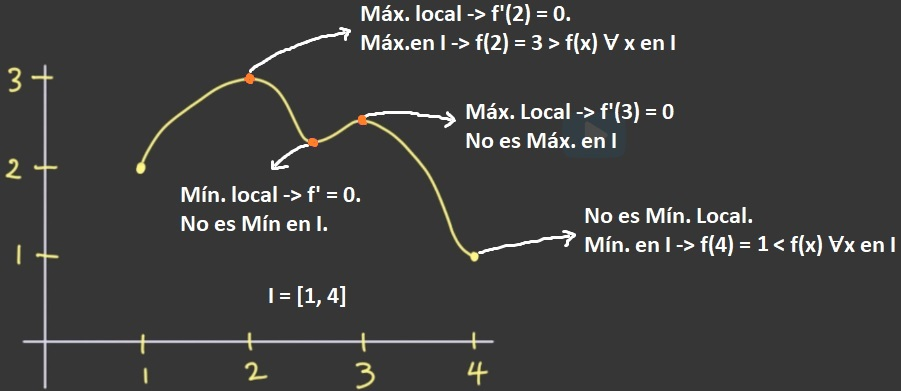
\includegraphics[scale=0.6]{img/min-max-interval.jpg}
\end{figure}

Como podemos observar, algunos puntos son extremos locales, pero no necesariamente corresponden al máximo o mínimo de la función en el intervalo $I$ y viceversa también, como vemos en el caso $x = 4$, donde $f(4)$ es el mínimo en el intervalo, pero no un mínimo local.

Ahora bien, nos hemos centrado en intervalos de valores donde la función es continua, pero sabemos que es posible encontrarnos con casos donde hay \textbf{discontinuidades}. Si, donde ocurre esto último caso, puede corresponder al máximo o mínimo de la función adentro del intervalo, entonces significa que \textbf{dicho valor no existe}, como lo vemos en la siguiente gráfica. También, como también se puede observar ahí, \textbf{es válido que haya más de un extremo en un intervalo}.

\begin{figure}[hbt!]
\centering
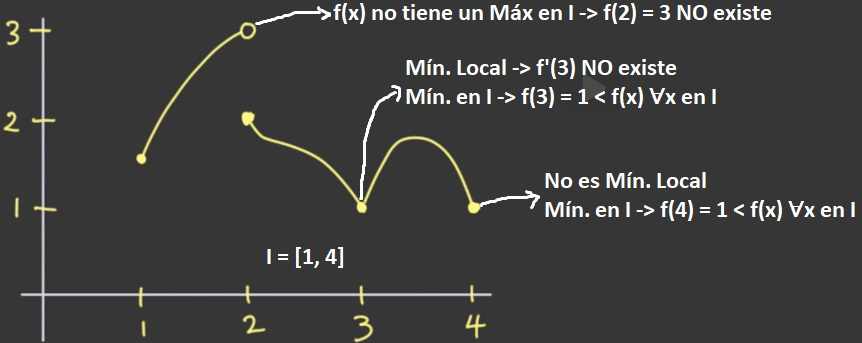
\includegraphics[scale=0.6]{img/min-max-interval-2.jpg}
\end{figure}

En otras palabras, \textbf{una función puede alcanzar su máximo o mínimo adentro de un intervalo $I$ en múltiples puntos o en ninguno}.


\subsubsection{Teorema del Valor Extremo.}

Para evaluar si una función tiene un máximo o mínimo adentro de un intervalo, usamos el \textbf{Teorema del Valor Extremo}, el cual señala que \textbf{podemos garantizar que alcanzará ambos extremos sí y solo sí es continua adentro de un intervalo cerrado $[a, \ b]$}.

Entonces, si una función $f$ es continua adentro de un intervalo $[a, \ b]$, podemos aplicar el \textbf{siguiente método} para hayar dónde se encuentran dichos máximos y mínimos.

\begin{enumerate}
\item Buscar los \textbf{puntos críticos de $f$ adentro del intervalo} y luego calcular el valor de la función en dichos lugares.

\item Calcular el \textbf{valor de la función en los puntos finales del intervalo}. Es decir, si el intervalo es $[a, \ b]$, entonces buscamos $f(a)$ y $f(b)$.

\item Evaluar en cuál de esos puntos $f$ alcanza su valor mínimo y máximo.
\end{enumerate}

\textbf{Ejercicio.} \quad Busque los valores máximos y mínimos de la función $g(x) = (3/2)x^{2/3} + x + 1$ para $-2 \leq x \leq 1$.

\textbf{Solución.} \quad Al ser $g(x)$ un polinomio, podemos asegurar que su dominio será $D = \mathbb{R}$. En otras palabras, es continua en dicho conjunto numérico y, por tanto, en $[-2, \ 1]$. Al serlo en ese tipo de intervalo, podemos garantizar a partir del teorema del valor extremo que existen valores máximos y mínimos en ese rango de números.

Luego, necesitamos buscar los puntos críticos de $g(x)$ y, para ello, debemos conocer su derivada, la cual tenemos a continuación.
\[
	g'(x) = \frac{1}{\sqrt[3]{x}} + 1
\]
De inmediato podemos señalar que un punto crítico es $x = 0$, puesto que se indetermina la derivada o, en otras palabras, ésta no existe. También podemos establecer que $g'(x) = 0$, para ver si hay valores de $x$ en donde se cumpla aquella igualdad.
\begin{align*}
	0 &= \frac{1}{\sqrt[3]{x}} + 1 \\
	x &= -1
\end{align*}
Por lo tanto, los puntos críticos de $g(x)$ son $(-1, \ 0)$, los cuales se encuentran dentro del intervalo $[-2, \ 1]$.

Finalmente, junto con los puntos finales del intervalo, $(-2, \ 1)$, veamos que valores toma $g(x)$ ahí y en donde se ubican sus puntos críticos, los cuales ilustramos en la siguiente tabla.

\begin{table}[hbt!]
\centering

\begin{tabular}{c | c c c c}
$x$ & $-2$ & $-1$ & $0$ & $1$ \\
\hline
$g(x)$ & $1.38$ & $1.5$ & $1$ & $3.5$
\end{tabular}

\end{table}

Entonces, podemos concluir que en el intervalo cerrado $[-2, \ 1]$, $g(x)$ alcanza su valor mínimo en $x = 0$ ($g(0) = 1$) y su máximo en $x = 1$ ($g(1) = 3.5$).



\subsubsection{Buscando Extremos en Intervalos que no son Cerrados.}

También es posible buscar los valores extremos de una función en un intervalo que no es cerrado. Es decir, sea de la forma $[a, \ b)$, $(-\infty, \ a]$, etc. La diferencia se da en que \textbf{el Teorema del Valor Extremo NO se aplica} en esos casos y, por consiguiente, \textbf{NO podemos garantizar si dicha función alcanza uno de los extremos o ambos}.

\newpage

En el caso de que \textbf{uno de los puntos finales (o ambos)} sea el $\pm \infty$, podemos evaluar su valor calculando su \textbf{límite al infinito} (págs. 13-15). Si existe el límite, usamos ese valor para calcular el \textit{output} de la función.

\textbf{Ejercicio.} \quad Adentro del intervalo $[0.5, \ \infty)$, busque los valores máximos y mínimos de la siguiente función:
\[
	g(x) = \frac{x^{2}}{2x^{3} + 1}
\]
\textbf{Solución.} \quad Si bien $g(x)$ es continua en $\mathbb{R}$, nos piden buscar sus valores extremos en un intervalo donde uno de sus puntos finales es abierto y al $\infty$. Por lo tanto, no podemos asegurar que exista uno o ambos extremos a partir del teorema del valor extremo.

Calculemos la derivada de $g(x)$. Aplicando la regla del cuociente, obtenemos que:
\[
g'(x) = \frac{(2x^{3} + 1)(2x) - (x^{2})(6x^{2})}{(2x^{3} + 1)^{2}}
	  = \frac{2x(1 - x^{3})}{(2x^{3} + 1)^{2}}
\]
A partir de $g'(x)$ podemos establecer que uno de sus puntos críticos será $x = 0$, debido a que el numerador se iguala a cero y, por tanto, toda la fracción. Sin embargo, no se encuentra incluido en el intervalo de nuestro interés, $[0.5, \ \infty)$, así que lo descartamos.

Para buscar otro punto crítico, podemos hacerlo evaluando en qué valores de $x$, $g'(x) = 0$.
\begin{align*}
0 &= \frac{2x(1 - x^{3})}{(2x^{3} + 1)^{2}} \\
0 &= 1 - x ^{3} \\
1 &= x
\end{align*}
El punto crítico $x = 1$ se encuentra en el intervalo, así que lo dejaremos para evaluarlo más adelante.

Luego, calculemos los valores que toma $g(x)$ en los puntos finales del intervalo. Cuando $x = 0.5$, $g(0.5) = 0.2$. Mientras que para el caso de $x = \infty$, debemos calcular el límite al infinito de $g(x)$ a medida que se acerca a dicho punto:
\[
\lim_{x \to \infty} \frac{x^{2}}{2x^{3} + 1} = 
\lim_{x \to \infty} \frac{1/x}{2 + (1/x^{3})} = 0
\]
Por lo tanto, a medida que $x \to \infty$, $g(x) \to 0$ o, en otras palabras, es asíntota horizontal en $x = 0$.

Finalmente, pongamos estos valores en una tabla para evaluar en qué valores se encuentran el máximo y/o mínimo de $g(x)$ en el intervalo $[0.5, \ \infty)$.

\begin{table}[hbt!]
\centering

\begin{tabular}{c | c c c}
$x$ & $0.5$ & $1$ & $\to \infty$ \\
\hline
$g(x)$ & $0.2$ & $\approx 0.33$ & $\to 0$
\end{tabular}

\end{table}

Como podemos apreciar, el valor máximo de $g(x)$ en el intervalo $[0.5, \ \infty)$ está en $x = 1$, pero si bien al acercarse al $\infty$ es cercano a $0$, nunca lo alcanza así que \textbf{podemos concluir que no tiene un valor mínimo adentro de dicho intervalo}.




\subsubsection{Problemas de Optimización.}

Al inicio de esta sección, señalamos que una aplicación del uso de dervivadas para buscar los extremos de una función en un intervalo, es para resolver problemas de optimización. Ahora veremos dos de ellos.

Algunos pasos que podemos seguir para resolver problemas de optimización, son:

\begin{enumerate}
\item Si es posible, dibujar un bosquejo del problema planteado.

\item Modelar una función que pueda servirnos para resolver el problema.

\item Definir un intervalo a partir de la información que nos entrega el problema.

\item Buscar el máximo y/o mínimo adentro de dicho intervalo.
\end{enumerate}

\textbf{Problema 1.} \quad Un campesino quiere construir un corral (\textit{pen}) rectangular para sus ovejas a un costado de su establo (\textit{barn}). Tal como se ve en el siguiente bosquejo, un lado del corral se forma con la muralla norte del establo, que mide 100 ft de largo, mientras que para los tres restantes se usarán cercas (\textit{fences}). El área del corral debe ser de $4000 \text{ ft}^{2}$.

\begin{figure}[hbt!]
\centering
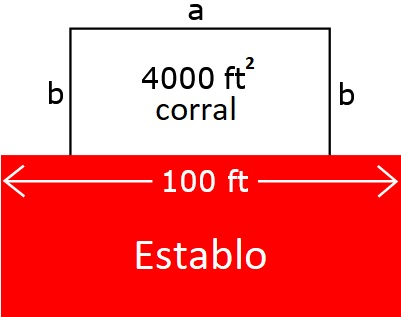
\includegraphics[scale=0.5]{img/opt-prob-1.jpg}
\end{figure}

Calcule el largo mínimo y máximo que deben alcanzar las cercas para que el campesino construya el corral para sus ovejas.

\newpage

\textbf{Solución.} \quad Ya tenemos un bosquejo del problema, así que podemos proceder a escribir una fórmula para el largo total de las cercas.

Si observamos bien, el largo total de las cercas está dado por el perímetro del corral, el cual es rectangular, pero sin considerar una cerca porque aquella está cubierta por la muralla norte del establo. Por otra parte, queremos conocer el largo total de las cercas a partir del largo mínimo y máximo que pueden alcanzar. En otras palabras, el perímetro del corral lo mediremos en función de su largo.

Por lo tanto, si establecemos que $a$ es el largo del corral, $b$ su ancho y el largo total está definido por $f(a)$, entonces:
\[
	f(a) = 2b + a
\]
Ahora, la idea es trabajar a partir de una sola variable, que en este caso es $a$. Lo que podemos hacer es definir $b$ en función de $a$ a partir del área del corral, que corresponde al área de un rectángulo, puesto que sabemos que es igual a $4000 \text{ ft}^{2}$ y conocemos dos de sus lados.
\begin{align*}
4000 \text{ ft}^{2} &= a \text{ ft } \cdot b \text{ ft } \\
\frac{4000}{a} \text{ ft} &= b
\end{align*}
De este modo, podemos redefinir $f(a)$ a partir de una sola variable.
\[
	f(a) = 2\left(\frac{4000}{a}\right) + a
\]
Luego, necesitamos definir un intervalo plausible con respecto al largo que puede alcanzar una cerca. Si imaginamos un poco, su medida máxima o mínima siempre deberá ser cualquier valor mayor a cero, pero como está adentro del establo, no podrá superar los 100 ft de largo\footnote{A una mayor longitud tendríamos que romper las murallas laterales xd.}. Por lo tanto, podemos establecer que el intervalo $I$ es:
\[
	I = (0, \ 100] \quad \text{o} \quad 0 < a \leq 100
\]
Como ya manejamos una función para medir el largo total de las cercas y un intervalo con respecto al mínimo y máximo que pueden alcanzar, estamos en condiciones de buscar los extremos de dicho intervalo.

\newpage

Comencemos calculando la derivada de $f(a)$.
\[
	f'(a) = 8000\left(\frac{1}{a}\right)' + 1
		  = 1 - \frac{8000}{a^{2}}
\]
Luego, busquemos los puntos críticos de $f(a)$. Uno de ellos puede ser $a = 0$, puesto que $f'(a)$ se indetermina o no existe $f'(0)$. Sin embargo, ya vimos en el intervalo que $a = 0$ no está considerado, así que lo descartamos. Otra forma para lograr este objetivo, es viendo en qué valores se cumple que $f'(a) = 0$.
\begin{align*}
0 &= 1 - \frac{8000}{a^{2}} \\
a^{2} &= 8000 \\
a &= \pm 40\sqrt{5}
\end{align*}
Como no estamos considerando valores menores a cero en nuestro intervalo, entonces solo dejamos como punto crítico a $a = 40\sqrt{5}$.

Finalmente, calculemos los valores que toma $f(a)$ en el punto crítico y en los valores finales del intervalo, en donde en $a = 0$ lo hacemos evaluando el límite de la función en dicho punto. Los resultados los tenemos en la siguiente tabla:

\begin{table}[hbt!]
\centering

\begin{tabular}{c | c c c}
$a$ & $\to 0^{+}$ & $40 \sqrt{5}$ & $100$ \\
\hline
$f(a)$ & $\to \infty$ & $\approx 179$ & $180$
\end{tabular}

\end{table}

Por lo tanto, en el intervalo $I = (0, \ 100]$, vemos que el largo total mínimo de la cerca para cubrir el área de $4000 \text{ ft}^{2}$ del corral, lo alcanzamos cuando $a = 40\sqrt{5}$ ft ($\approx 179$ ft), pero no es posible conocer en qué valor logra su máximo porque $f(a) \to \infty$ cuando $a \to 0^{+}$. Lo cual es razonable, porque nuestra idea es optimizar en cuanto a lo que menos necesitamos. Es decir, al largo mínimo para cubrir un área determinada.

Para verificar si estamos en lo correcto en que el largo mínimo que puede alcanzar una cerca es en $a = 40\sqrt{5}$, podemos calcular el área del corral y ver si se cumple que es igual a $4000 \text{ ft}^{2}$.
\begin{align*}
4000 \text{ ft}^{2} &= a \cdot b \ (\text{ft}^{2}) \\
4000 \text{ ft}^{2} &=
	40\sqrt{5} \cdot \left(\frac{4000}{40\sqrt{5}}\right) \
	(\text{ft}^{2}) \\
4000 \text{ ft}^{2} &= 4000 \text{ ft}^{2}
\end{align*}

\newpage

\textbf{Problema 2.} \quad Supongamos que tenemos 100 pulgadas de alambre y queremos cortarlo en dos piezas. Una la usaremos para hacer un círculo y con la otra haremos un cuadrado.

Sean $c$ el perímetro del círculo y $s$ el perímetro del cuadrado ($s$ de \textit{square}), calcule: (1) el área total de las dos formas en función de $c$ y (2) los valores de $c$ para minimizar y maximizar dicha área.

\textbf{Solución.} \quad Primero comencemos dibujando un bosquejo, el cual hice de la siguiente manera\footnote{¿Podría haber sido de otra forma? Sí, pero solo se me ocurrió de esta manera xd.}.

\begin{figure}[hbt!]
\centering
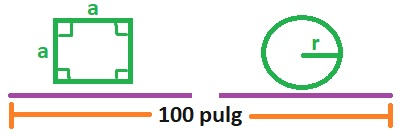
\includegraphics[scale=0.7]{img/opt-prob-2.jpg}
\end{figure}

Una idea que nos entrega el bosquejo y el problema, es que el perímetro de ambas figuras son dependientes entre sí, porque se forman del mismo alambre. En consecuencia una medida está en función de la otra, lo cual podemos describirlo matemáticamente.
\begin{align*}
c + s &= 100 & c + s &= 100 \\
s &= 100 - c & c &= 100 - s
\end{align*}
Lo anterior también va para el área total de ambas figuras, el cuál denotaremos como $A_{T}$, que será la suma entre las áreas del círculo $A_{c}$ y del cuadrado $A_{s}$.
\begin{align*}
A_{T} &= A_{c} + A_{s} \\
      &= \pi r^{2} + a^{2}
\end{align*}
Ahora, tenemos dos problemas: el primero es que necesitamos conocer el radio $r$ del círculo y el lado $a$ del cuadrado y, en segundo lugar, que el $A_{T}$ esté en función de $c$.

Lo primero, podemos conocerlo a partir de las fórmulas de los perímetros que vimos arriba. Reemplacemos los lados izquierdos de ambas ecuaciones con sus respectivas fórmulas y despejemos tanto el lado $a$ del cuadrado como el radio $r$ del círculo.
\begin{align*}
4a &= 100 - c & 2\pi r &= 100 - s \\
a &= \frac{100-c}{4} & r &= \frac{100-s}{2\pi}
\end{align*}

\newpage

Luego, reemplacemos $a$ y $r$ en la fórmula de $A_{T}$.
\begin{align*}
A_{T} &= \pi \left(\frac{100-s}{2\pi}\right)^{2} + 
         \left(\frac{100-c}{4}\right)^{2} \\
      &= \frac{(100-s)^{2}}{4\pi} + 
         \left(\frac{100-c}{4}\right)^{2}
\end{align*}
En la primera pregunta nos piden el $A_{T}$ en función de $c$, el cual denotaremos como $A(c)$ y estableceremos que $A_{T} = A(c)$.
\[
A(c) = \frac{(100-s)^{2}}{4\pi} + \left(\frac{100-c}{4}\right)^{2}
\]
Pero, como vemos, tenemos el problema de tener a $s$ en la fórmula de $A(c)$. Sin embargo, anteriormente establecimos que el perímetro del círculo en función de $s$, es $c = 100 - s$, por lo tanto podemos reemplazarlo en el numerador de la fracción de la izquierda de la fórmula y \textbf{obtenemos así la respuesta (1)}.
\[
	A(c) = \frac{c^{2}}{4\pi} + \left(\frac{100-c}{4}\right)^{2}
\]
Teniendo la fórmula, ahora podemos proceder a buscar los valores de $c$ que nos sirven para minimizar o maximizar $A(c)$.

Partamos definiendo el intervalo. Recordemos que ambos perímetros, $c$ y $s$, dependen uno del otro porque se forman del mismo alambre de 100 pulgadas de largo. En ese sentido, podemos decir que $c = 100$ cuando $s = 0$, del mismo modo, $s = 100$ cuando $c = 0$. Esto significa que el perímetro $c$ puede tomar valores desde $0$ hasta $100$, por lo tanto podemos definir su intervalo $I$ como:
\[
	I = [0, \ 100] \quad \text{o} \quad 0 \leq c \leq 100
\]
Luego, busquemos los puntos críticos a partir de la derivada de $A(c)$. Al calcularla, obtenemos que:
\[
	A'(c) = \frac{c}{2\pi} - \frac{100-c}{8}
\]

\newpage

Como en ningún valor de $c$ se indetermina $A'(c)$, entonces veamos en qué valores de dicho perímetro, esta derivada se iguala a cero.
\begin{align*}
0 &= \frac{c}{2\pi} - \frac{100-c}{8} \\
\frac{100 - c}{8} &= \frac{c}{2\pi} \\
100 - c &= \frac{4}{\pi} c \\
100 &= \frac{4}{\pi} c + c \\
\frac{100 \pi}{4 + \pi} &= c \\
c &\approx 43.99
\end{align*}
Finalmente, calculemos los valores que toma $A(c)$ en los extremos del intervalo $I$ como en el punto crítico que acabamos de obtener.

\begin{table}[hbt!]
\centering

\begin{tabular}{c | c c c}
$c$ & $0$ & $\approx 43.99$ & $100$ \\
\hline
$A(c)$ & $625$ & $\approx 350.06$ & $\approx 795.77$
\end{tabular}

\end{table}

Por lo tanto, \textbf{nuestra respuesta a la pregunta (2), es la siguiente}: En función del perímetro del círculo, el área total de las dos figuras, $A(c)$, podemos minimizarla (alcanzar su mínimo óptimo) cuando $c \approx 43.99$ y maximizarla (alcanzar su máximo óptimo) cuando $c = 100$.




\subsection{Problemas de Tasas Relacionadas.}

En esta última sección, revisaremos situaciones donde conocemos una tasa de cambio y buscamos conocer otra que está vinculada a la primera. A este tipo de problemas se los conoce como \textbf{problemas de tasas relacionadas} (o vinculadas).

En particular, nos referimos a tasas de cambios instantáneas que, como ya sabemos, es otra forma de referirnos a las derivadas. Como veremos, dos tasas estarán vinculadas y podremos conocer la que nos interesa \textbf{derivando implícitamente} posterior a haber establecido el modelo o función que explica el problema a estudiar.

Para resolver este tipo de problemas, podemos seguir la siguiente estrategia:

\begin{enumerate}
\item Dibujar un bosquejo del problema.

\item Identificar las variables y tasas relevantes.

\item Buscar una ecuación que vincule a las variables relevantes que siempre se mantengan.

\item Derivar implícitamente la ecuación.

\item Reemplazar las variables de la ecuación con los valores dados o los obtenidos y resolverla.
\end{enumerate}

\textbf{Problema 1.} \quad Un barco de carga de petróleo ha sufrido una ruptura y está derramando su contenido al océano a 2 millones de litros por hora. Es posible modelar el derrame como un cilindro muy delgado, cuyo volumen está dado por $V = \pi h r^{2}$, donde $r$ es el radio del derrame y $h$ su altura o grosor. Supongamos que el valor de $h$ se mantiene constante en $2$ cm. Por otra parte, al momento de estar resolviendo este problema, el radio del derrame es de $250$ m. Con esta información, calculemos la velocidad con que se expande el perímetro externo del derrame.

\textbf{Solución.} \quad Sigamos la estrategia vista y partamos dibujando un bosquejo del problema. En particular, centrémonos en el cilindro delgado de petróleo que se está formando en el océano.

\begin{figure}[hbt!]
\centering
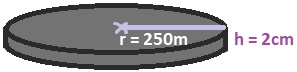
\includegraphics[scale=0.7]{img/related-prob-1.jpg}
\end{figure}

Veamos ahora la información básica que manejamos:

\begin{itemize}
\item $V = \pi h r^{2}$.
\item $h = 2$ cm (constante).
\item $r = 250$ m (al momento).
\end{itemize}

Por otra parte, al leer podemos darnos cuenta que tenemos dos tasas a la vista: la cantidad de petróleo que se derrama por hora y la velocidad con que se expande el perímetro externo del derrame.

La cantidad de petróleo que sale del barco, es medida en litros por hora. Como el litro es una medida de volumen, entonces podemos asumir que aquella tasa es la derivada del volumen con respecto a un tiempo $t$, medido en horas:
\[
	\frac{d}{dt}V = 2 \cdot 10^{6} \text{ lt/hr}
\]
La velocidad de expansión del perímetro del derrame también es una tasa de cambio, que podemos entenderla como la distancia con que avanza en un período de tiempo determinado. Como su base es circular, podemos asumir que dicha distancia está dada por el radio $r$. Por lo tanto, esta tasa corresponde a la derivada de $r$ con respecto a un tiempo $t$ y es la medida que buscamos conocer.
\[
	\frac{d}{dt}r = \text{?}
\]
Por lo tanto, nuestras variables relevantes en este problema son el volumen $V$ y el radio $r$.

Ahora bien, tenemos que ver cómo calculamos $dr/dt$. La fórmula que manejamos\footnote{Y que, por tanto, no necesitamos modelar.} es la del volumen del cilindro, puesto que a partir de esa figura ha sido modelado el problema.
\[
	V = \pi h r^{2}
\]
Sabemos que tenemos que derivar. No es buena idea hacerlo despejando en la ecuación a $r$ o a $V$, para luego derivarlas con respecto a una u otra variable, porque nos tomaría mucho tiempo. En vez de aquello, lo que podemos hacer es \textbf{derivarla implícitamente}, aprovechando que ambas tasas se miden con respecto a una variable, que en este caso es $t$. Por lo tanto, podemos establecer que:
\[
	\frac{d}{dt}V = \frac{d}{dt}(\pi h r^{2})
\]
Antes de derivar el lado derecho, debemos tener muy presente en este caso que si bien $h$ es constante, $r$ no lo es. Nos dicen que el radio \textbf{en ese momento} es de $250$ m, pero sabemos que sigue expandiéndose. Por lo tanto, dicho valor lo incluiremos después de haber calculado la derivada porque, de lo contrario, estaremos calculando su derivada solo para ese momento.

Procedamos a calcular implícitamente las derivadas de la ecuación.
\begin{align*}
	\frac{d}{dt}V &= \frac{d}{dt}(\pi h r^{2}) \\
	\frac{d}{dt}V &= \pi h \frac{d}{dr} r^{2} \cdot \frac{d}{dt} r \\
	\frac{d}{dt}V &= \pi h 2r \cdot \frac{d}{dt} r \\
	\frac{dV/dt}{\pi h 2r} &= \frac{d}{dt} r
\end{align*}

\newpage

Ahora solo debemos reemplazar los valores del lado derecho para obtener $dr/dt$. No olvidemos que los valores tienen sus propias unidades de medidas. Como el radio lo estamos midiendo en metros, todas las medidas las pasaremos a dicha unidad\footnote{$1 \text{ lt} = 0.001 \text{ m}^{3}$ y $1 \text{ cm} = 0.01 \text{ m}$}.
\begin{align*}
\frac{d}{dt}V &= \frac{2 \cdot 10^{6}}{1 \cdot 10^{3}}
				 \frac{\text{m}^{3}}{\text{hr}} 
		       = 2 \cdot 10^{3} \frac{\text{m}^{3}}{\text{hr}} \\ \\
h &= \frac{2}{100} = 2 \cdot 10^{-2} \text{ m}
\end{align*}
También escribamos $r = 2.5 \cdot 10^{2}$ m, para ser consistente en que estamos trabajando con notación científica (para hacerlo más fácil).

Por lo tanto, al reemplazar $r$, $dV/dt$ y $h$, podemos obtener $dr/dt$:
\begin{align*}
% Se lee feito, peldón :(
\frac{d}{dt} r &= \frac{2 \cdot 10^{3}}{
					    2 \pi (
					      2 \cdot 10^{-2} \cdot 2.5 \cdot 10^{2}
					    )
					   }
				  \left(
				    \frac{\text{m}^{3}/\text{hr}}{\text{m}^{2}}
				  \right)
               = \frac{200}{\pi} \text{ (m/hr)}
\end{align*}
En otras palabras, el perímetro externo del derrame de petróleo se expande a una velocidad de $200/\pi$ m/hr sobre el océano.


\textbf{Problema 2.} \quad En un edificio está ocurriendo un incendio y un camión de bomberos se encuentra en el lugar para realizar tareas de rescate.

Como se ve en la imagen de abajo, el camión se encuentra retrocediendo hacia el edificio, y lo hace a 0.5 pies (\textit{feet} o ft) por segundo.

\begin{figure}[hbt!]
\centering
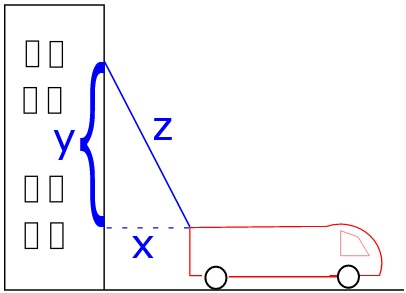
\includegraphics[scale=0.5]{img/related-prob-2.jpg}
\end{figure}

También se puede apreciar que la escalera del camión de bomberos se encuentra ubicada a un costado del edificio, la cual se alarga a una velocidad de 0.2 pies por segundo y comienza desde la parte trasera del vehículo, a 6 pies de altura.

\newpage

Al alargarse por completo la escalera del camión y cuando el vehículo se encuentra a 7 pies de distancia del edificio, ésta chocará con una gárgola de 30 pies de altura. Nuestro objetivo es saber la velocidad con que se moverá la parte superior de la escalera a medida que se acerca el camión al edificio.

\textbf{Solución.} \quad Ya tenemos un bosquejo del problema, así que veamos las variables y tasas que son relevantes, así como la información que nos entregan sobre ellas y aprovecharemos las letras ubicadas en aquel dibujo para definir las variables.

En primer lugar, nos indican que el camión está retrocediendo a una velocidad determinada. Es decir, es una tasa que está en función de un tiempo $t$ y se mueve en la dirección de $x$. Por lo tanto, corresponde a $dx/dt$, pero debemos tener presente que se está moviendo \textbf{en sentido contrario}, lo que implica que su valor será de signo \textbf{negativo}. En otras palabras, $dx/dt = -0.5$ ft/seg.

Otra tasa que podemos apreciar, corresponde a la velocidad con la que se alarga la escalera del camión. Su distancia está dada en el bosquejo por $z$ y, como está en función de un tiempo $t$, podemos establecer que $dz/dt = 0.2$ ft/seg.

Otra información relevante que nos entrega el problema, es que la distancia entre el suelo y dónde comienza la escalera del camión, es de 6 ft. También que desde el piso hasta dónde toca la escalera al costado del edificio, hay 30 ft y eso ocurre cuando el camión se encuentra a 7ft del inmueble. Todo esto podemos llevarlo al bosquejo para visualizarlo mejor.

\begin{figure}[hbt!]
\centering
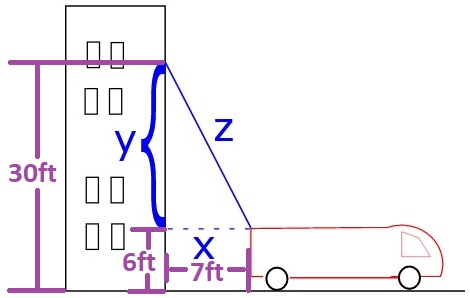
\includegraphics[scale=0.5]{img/related-prob-2b.jpg}
\end{figure}

A partir de esta información podemos establecer que:
\begin{align*}
y + 6 \text{ ft} &= 30 \text{ ft} \\
y &= 24 \text{ ft}
\end{align*}

\newpage

Y también se puede apreciar que entre la distancias de $x$, $y$ y $z$ se forma un triángulo rectángulo. Por consiguiente, podemos calcular el valor de $z$ por medio del teorema de Pitágoras.
\begin{align*}
z &= \sqrt{x^{2} + y^{2}} \\
 &= \sqrt{(7^{2} + 24^{2})(\text{ft}^2)} \\
z &= 25 \text{ ft}
\end{align*}
Finalmente, nos preguntan por la velocidad con la que se mueve la parte superior la escalera a medida que retrocede el camión. Éste corresponde al movimiento vertical de la escalera, el cual está dado por $y$. Al ser una velocidad, dicha tasa también está en función de un tiempo $t$, de manera que nos están pidiendo calcular $dy/dt$.

Ahora bien, a diferencia del problema anterior, no nos dan una ecuación que modele el ejercicio. No obstante, acabamos de ver que todo este caso se está siguiendo geométricamente un triángulo rectángulo\footnote{De este modo, por ejemplo, calculamos $z$.}. En consecuencia, podemos modelarlo a partir de esta figura y la ecuación que podemos usar para encontrar $dy/dt$, es la dada por el teorema de Pitágoras. Es decir:
\[
	x^{2} + y^{2} = z^{2}
\]
En ese sentido, lo que haremos es derivar implícitamente toda esta ecuación en función de $t$.
\begin{align*}
	\frac{d}{dt} (x^{2} + y^{2}) &= \frac{d}{dt}z^{2} \\
	2x\frac{d}{dt}x + 2y\frac{d}{dt}y &= 2z \frac{d}{dt}z	
\end{align*}
Si factorizamos por $2$ el lado izquierdo y, posteriormente, despejamos $dy/dt$, obtenemos la siguiente ecuación:
\[
 \frac{d}{dt}y = \frac{z(dz/dt) - x(dx/dt)}{y}
\]
Ya conocemos los valores que toman cada variable y tasa del lado derecho, así que simplemente los reemplazamos y calculamos $dy/dt$.
\begin{align*}
	\frac{d}{dt}y &= \frac{25 \cdot 0.2 - 7 \cdot(-0.5)}{24} \\
	              &= \frac{17}{24} \\
	\frac{d}{dt}y &\approx 0.71 \text{ ft/seg}
\end{align*}
Por lo tanto, cuando el camión de bomberos retrocede acercándose al edificio, la parte superior de la escalera se mueve a una velocidad de $\approx 0.71$ ft/seg.


\textbf{Problema 3.} \quad Una persona de 6 ft de alto está caminando por la calle. Directamente atrás suyo, se encuentra un poste de luz de 10 ft de alto que proyecta una sombra sobre el suelo.

\begin{figure}[hbt!]
\centering
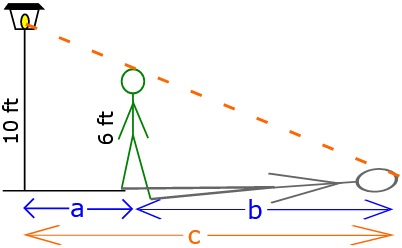
\includegraphics[scale=0.6]{img/related-prob-3.jpg}
\end{figure}

Cuando la persona está parada y detenida, se encuentra a 40 ft del poste de luz. Por otra parte, al momento en que la punta de la sombra la sobre pasa, lo hace a 3 ft/seg. Calcule qué tan rápido camina dicha persona.

\textbf{Solución.} \quad Este problema es similar al anterior, puesto que también nos dan el bosquejo del problema, pero no una fórmula que nos permita modelarla, pero veremos que el dibujo será suficiente para lograr ese objetivo.

Además de la información sobre las alturas de la persona y del poste (6ft y 10ft, respectivamente), más implícitamente nos entregan información sobre dos tasas. Una de ellas es la rapidez con que avanza la punta de la sombra. Si observamos el bosquejo, podremos apreciar que su distancia es aquella entre el poste y donde se ubica la cabeza de la sombra de la persona. Es decir, corresponde a $c$. Por lo tanto, es posible señalar que:
\[
	\frac{d}{dt}c = 3 \text{ ft/seg}
\]
La otra tasa que nos indican y que también es la que buscamos calcular, es la rapidez con que camina la persona. Si calculamos su distancia como la diferencia entre el lugar donde se encuentra y la ubicación del poste, podemos decir que es igual a $a$. En consecuencia, su tasa de cambio instantánea con respecto a un tiempo $t$ corresponde a:
\[
	\frac{d}{dt}a = \text{? ft/seg}
\]
Ahora bien, necesitamos modelar una ecuación para conocer $da/dt$ y, para ello, nos ayudaremos del bosquejo.

Al observar el bosquejo con mayor detalle, entre el poste de luz, la persona, su sombra y la luz que se proyecta desde el foco del primero, se forman dos triángulos rectángulos que son semejantes\footnote{Creo que es $LLA$ o $ALL$. No lo recuerdo bien xd.}.

\begin{figure}[hbt!]
\centering
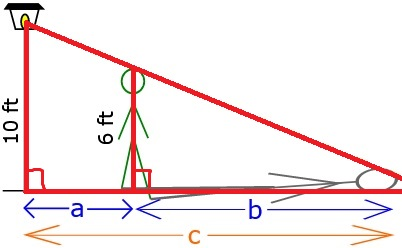
\includegraphics[scale=0.6]{img/related-prob-3b.jpg}
\end{figure}

En ese sentido, podemos establecer la siguiente relación:
\[
	\frac{c}{10} = \frac{b}{6}
\]
Nos interesa trabajar tanto con las tasas de $c$ como de $a$. En ese sentido, podemos establecer que $b = c - a$. Por lo tanto:
\[
	\frac{c}{10} = \frac{c - a}{6}
\]
Luego, simplemente despejamos $a$ de la ecuación.
\begin{align*}
	\frac{c}{10} &= \frac{c - a}{6} \\
	6c &= 10(c - a) \\
	\frac{2}{5}c &= a
\end{align*}
Finalmente, calculamos la derivada con respecto a $t$ en ambos lados de la ecuación.
\begin{align*}
	\frac{d}{dt}\left(\frac{2}{5}c\right) &= \frac{d}{dt}a \\
	\frac{2}{5} \left(\frac{d}{dt} c\right) &= \frac{d}{dt} a
\end{align*}
Sabemos que $dc/dt = 3$ ft/seg. Por consiguiente:
\begin{align*}
	\frac{2}{5} \cdot 3 \text{ ft/seg} &= \frac{d}{dt} a \\
	1.2 \text{ ft/seg} &= \frac{d}{dt} a
\end{align*}

\newpage

En otras palabras, la persona camina a una rapidez de $1.2$ ft/seg.

Algo llamativo de este problema es que para resolverlo, no tuvimos que usar la distancia entre el poste y la persona cuando se encontraba estacionada, que era igual a 40 ft. Es decir, era un problema más sencillo del que uno podría pensar.

\end{document}